\chapter{Implementierung} \label{cha:Implementierung}

In diesem Kapitel soll das zuvor vorgestellte Verfahren implementiert werden. Zuerst wird die experimentelle Umgebung auf dem PC, einschließlich der benutzten Geräte, und die Software vorgestellt. Anschließend die Implementierung der beiden vorherigen Methoden mit Matlab, welche die Anzeige jedes Schritt und dessen Demonstration der Endergebnisse enthalten. Schließlich läuft die Implementierung des Detektionsverfahrens auf einer Smartphone-GPU.

\section{Experiment Umgebung}

Hier wird die Experimentumgebung auf PC-Seite bzw. Test Geräte, Software in diese Arbeit erläutert. Google Pixel wird benutzt, um die Bild aufzunehmen. Dessen Parameter sind in Tabelle \ref{tbl:Parameter der Kameras im Vergleich} verfügbar. Die Anwendungssoftware $ ``VLCReceiver" $ wird mit automatischer Einstellungsmodus benutzt. Entsprechend dem möglichen Einsatzbereich des David-Systems wurden im Experiment die Bildschirme mit verschiedener Größen und Umgebungen ausgewählt. Die in dem Experiment verwendeten Bildschirme sind in der Tabelle \ref{tbl:Verwendeter Bildschirm} gezeigt. Die aufgenommen Bilder wird auf der PC-Seite mit Matlab 2017b unter der Lizenz der TU Dortmund verarbeitet.

\begin{table}[htb]
	\captionabove{Verwendeter Bildschirm}
	\label{tbl:Verwendeter Bildschirm}
	\footnotesize
	\centering
	\rowcolors{2}{white}{gray!25}	%TUgreen!25
	%\begin{tabular}{|p{3cm}|p{2cm}|p{2cm}|p{2cm}|p{2cm}|p{2cm}|}	%p{}m{}b{}clr
	\begin{tabular}{|c|c|c|c|c|c|}
	\toprule
	\textbf{Hersteller} & \textbf{Model} & \textbf{Beleuchtung} & \textbf{Auflösung} & \textbf{Größe}	& \textbf{Frequenz}\\
	\midrule
	Lenovo Laptop & T440P & LED & $ 1920 \times 1280$ & 14'' & 60 \\
	Samsung 	  & SMB2440MH   & LED & $ 1920 \times 1280$ & 24'' & 60 \\
	Ausu  		  & VG248   & LCD & $ 1920 \times 1280$ & 24'' & 60 \\
	LG  		  & 55EF950V & OLED & $ 2160 \times 3840$ & 55'' & 120 \\
	 Projektor & 1234 & 1234 & 1920 & 14'' & 60 \\
	
	\bottomrule
	\end{tabular}
\end{table} 

\section{Implementierung der ersten Verfahren}
Hier ist der Implementierungsprozess von Methode 1. Das Bild stammt aus einer Reihe von  achten Bildern, die mit einer Smartphone in Handy aufgenommen wurden. Entsprechend den Eigenschaften von Bildregistration in dieser Arbeit sind die von der handgehaltenen Kamera aufgenommenen Objekte alle statische Videos. Dies bedeutet, dass sich der Inhalt des Videos nicht ändert. Im tatsächlichen Betrieb entspricht es einer statischen elektronischen Werbetafel. Die Modulationsamplitude werden als 6 erstellt, anschließend Daten Datenblock als $ 4 \times 4 Pixel$, QR Muster Größe  als $ 72 \times 72 Pixel$.

Aufgrund von Handschütteln während der Aufnahme entsteht eine leichte Verschiebung zwischen den Bildern. Um diese Effekt deutlicher anzuzeigen, wird das erste Bild und das achte Bild zum Vergleich verwendet, wie in Abbildung \ref{fig:vorregistration} zeigt. 
%Die durchschnittliche Entfernung der entsprechenden Pixel zwischen den zwei Bildern beträgt ca.2 Pixel. 
Abbildung \ref{fig:nachregis} zeigt das Bild nach der Bildregistration. Wie zu sehen ist, ist der Abstand gut komprimiert. %Die durchschnittliche Entfernung hier beträgt ca. 0.45 Pixel.
 
\begin{figure}[H]
\centering 
\begin{minipage}[b]{0.49\textwidth} 
\centering 
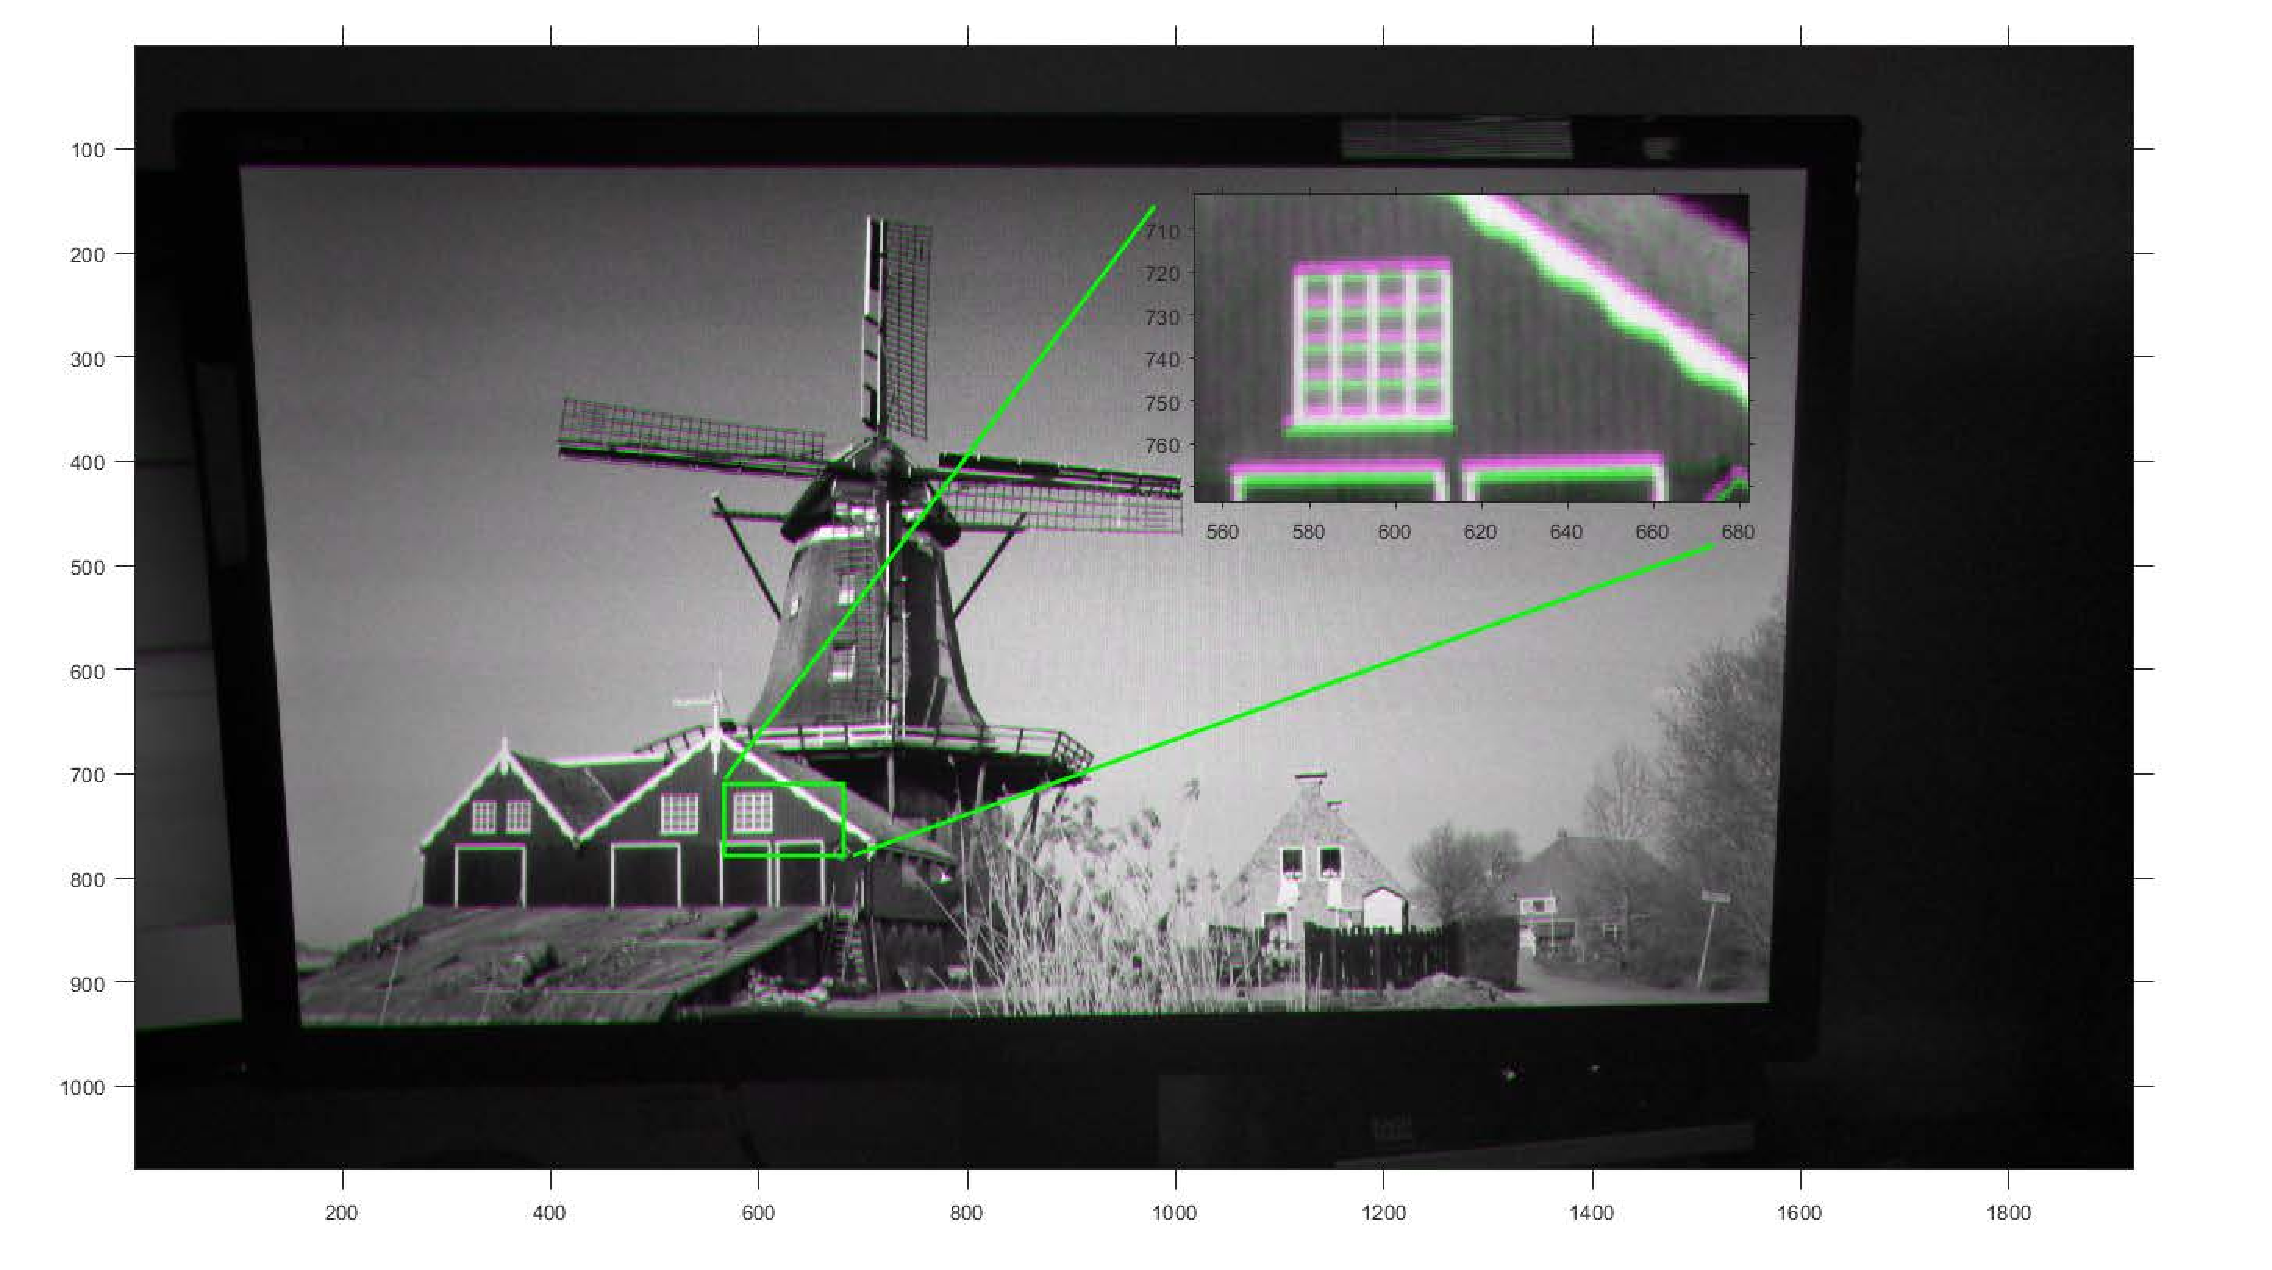
\includegraphics[width=1.0\textwidth]{images/5_Implementirung/vorregistration.pdf} 
\caption{Bilder vor Bildregistration}
\label{fig:vorregistration}
\end{minipage}
\begin{minipage}[b]{0.49\textwidth} 
\centering 
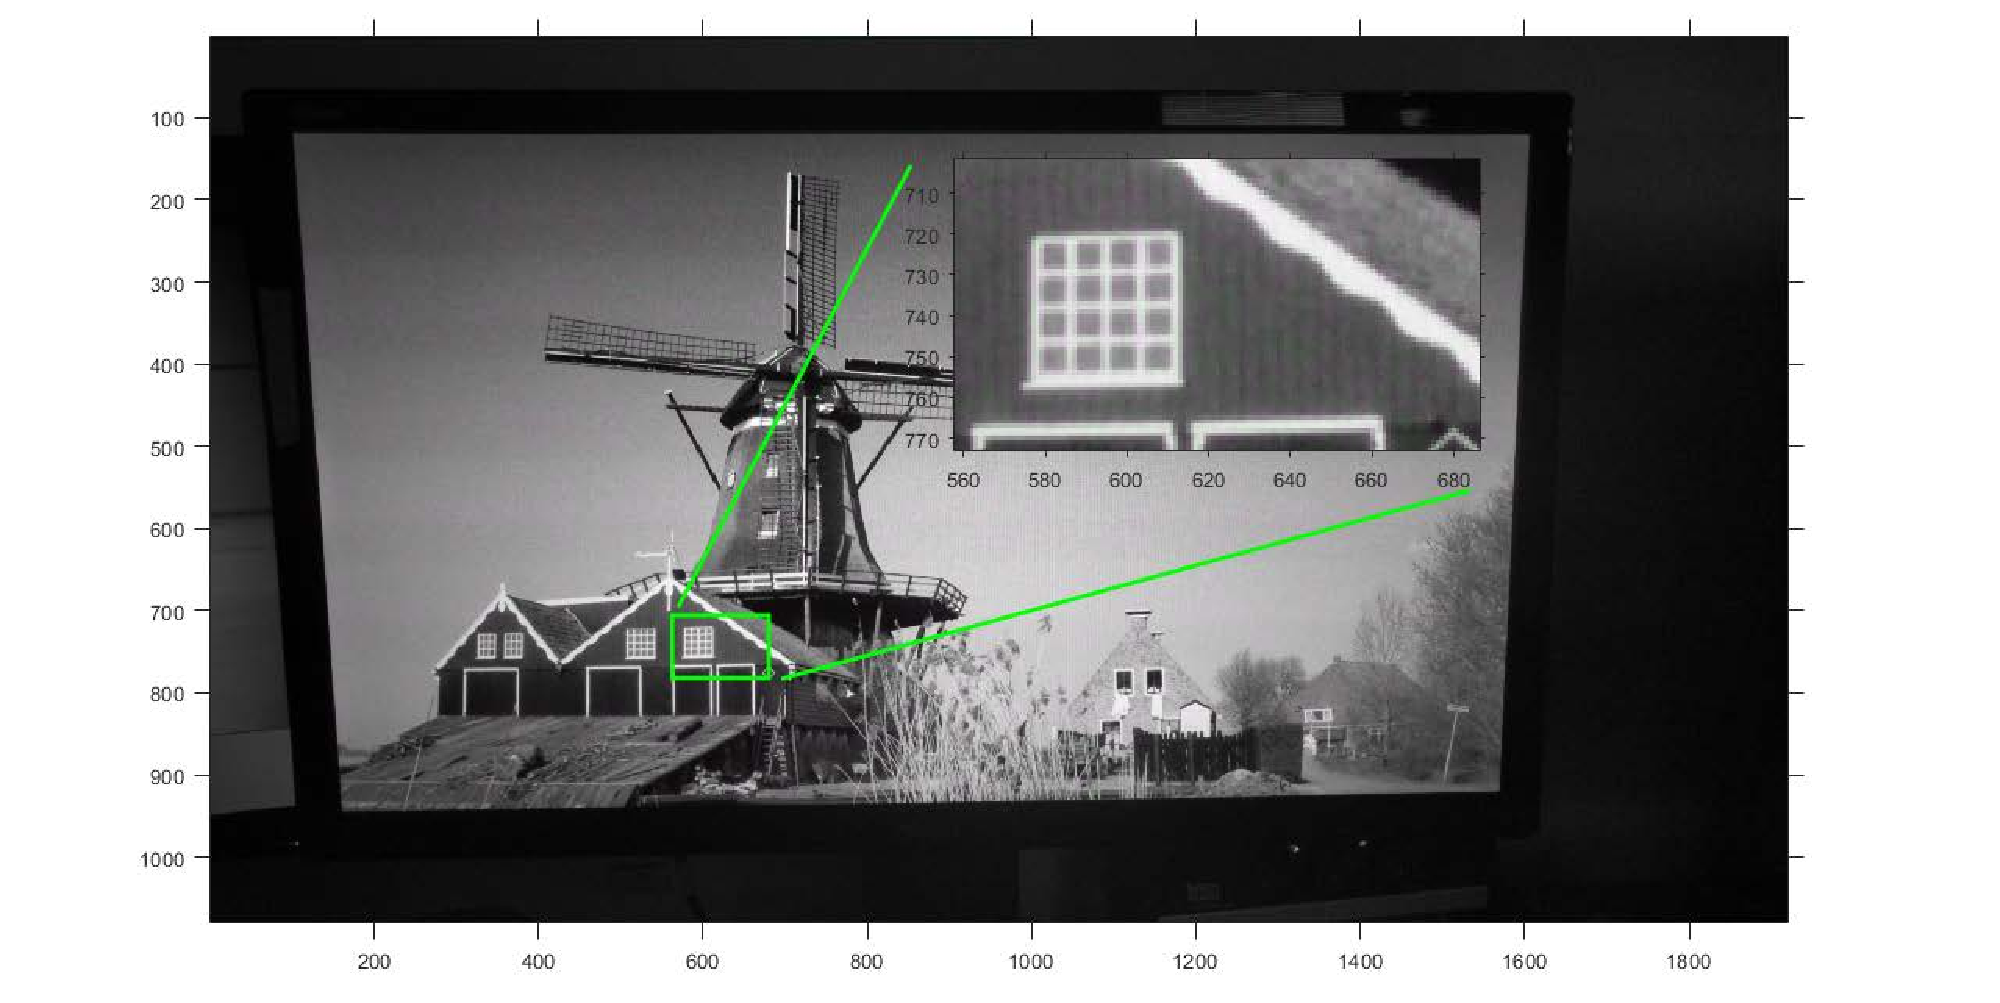
\includegraphics[width=1.1\textwidth]{images/5_Implementirung/nachregis.pdf}
\caption{Bilder nach Bildregistration}
\label{fig:nachregis}
\end{minipage}
\end{figure}
 
Aufgrund der verschiedene Bildwiederholfrequenz werden die QR Muster in den Differenzbildern einige unerwartete Effekte aufweisen könnten, wie in Tabelle 3.2 gezeigt. Um diese zu lösen, eine Absolutwertoperation wird durchführt. Danach mit Hilfe des Berechnung der $ ``Enegie" $ jedes Differenzbild lassen sich ein neu zu detektierendes Bild entstehen. Es wird in Abbildung \ref{fig:nachdiff} gezeigt.

\begin{figure}[H]
\centering 
\begin{minipage}[b]{0.49\textwidth} 
\centering 
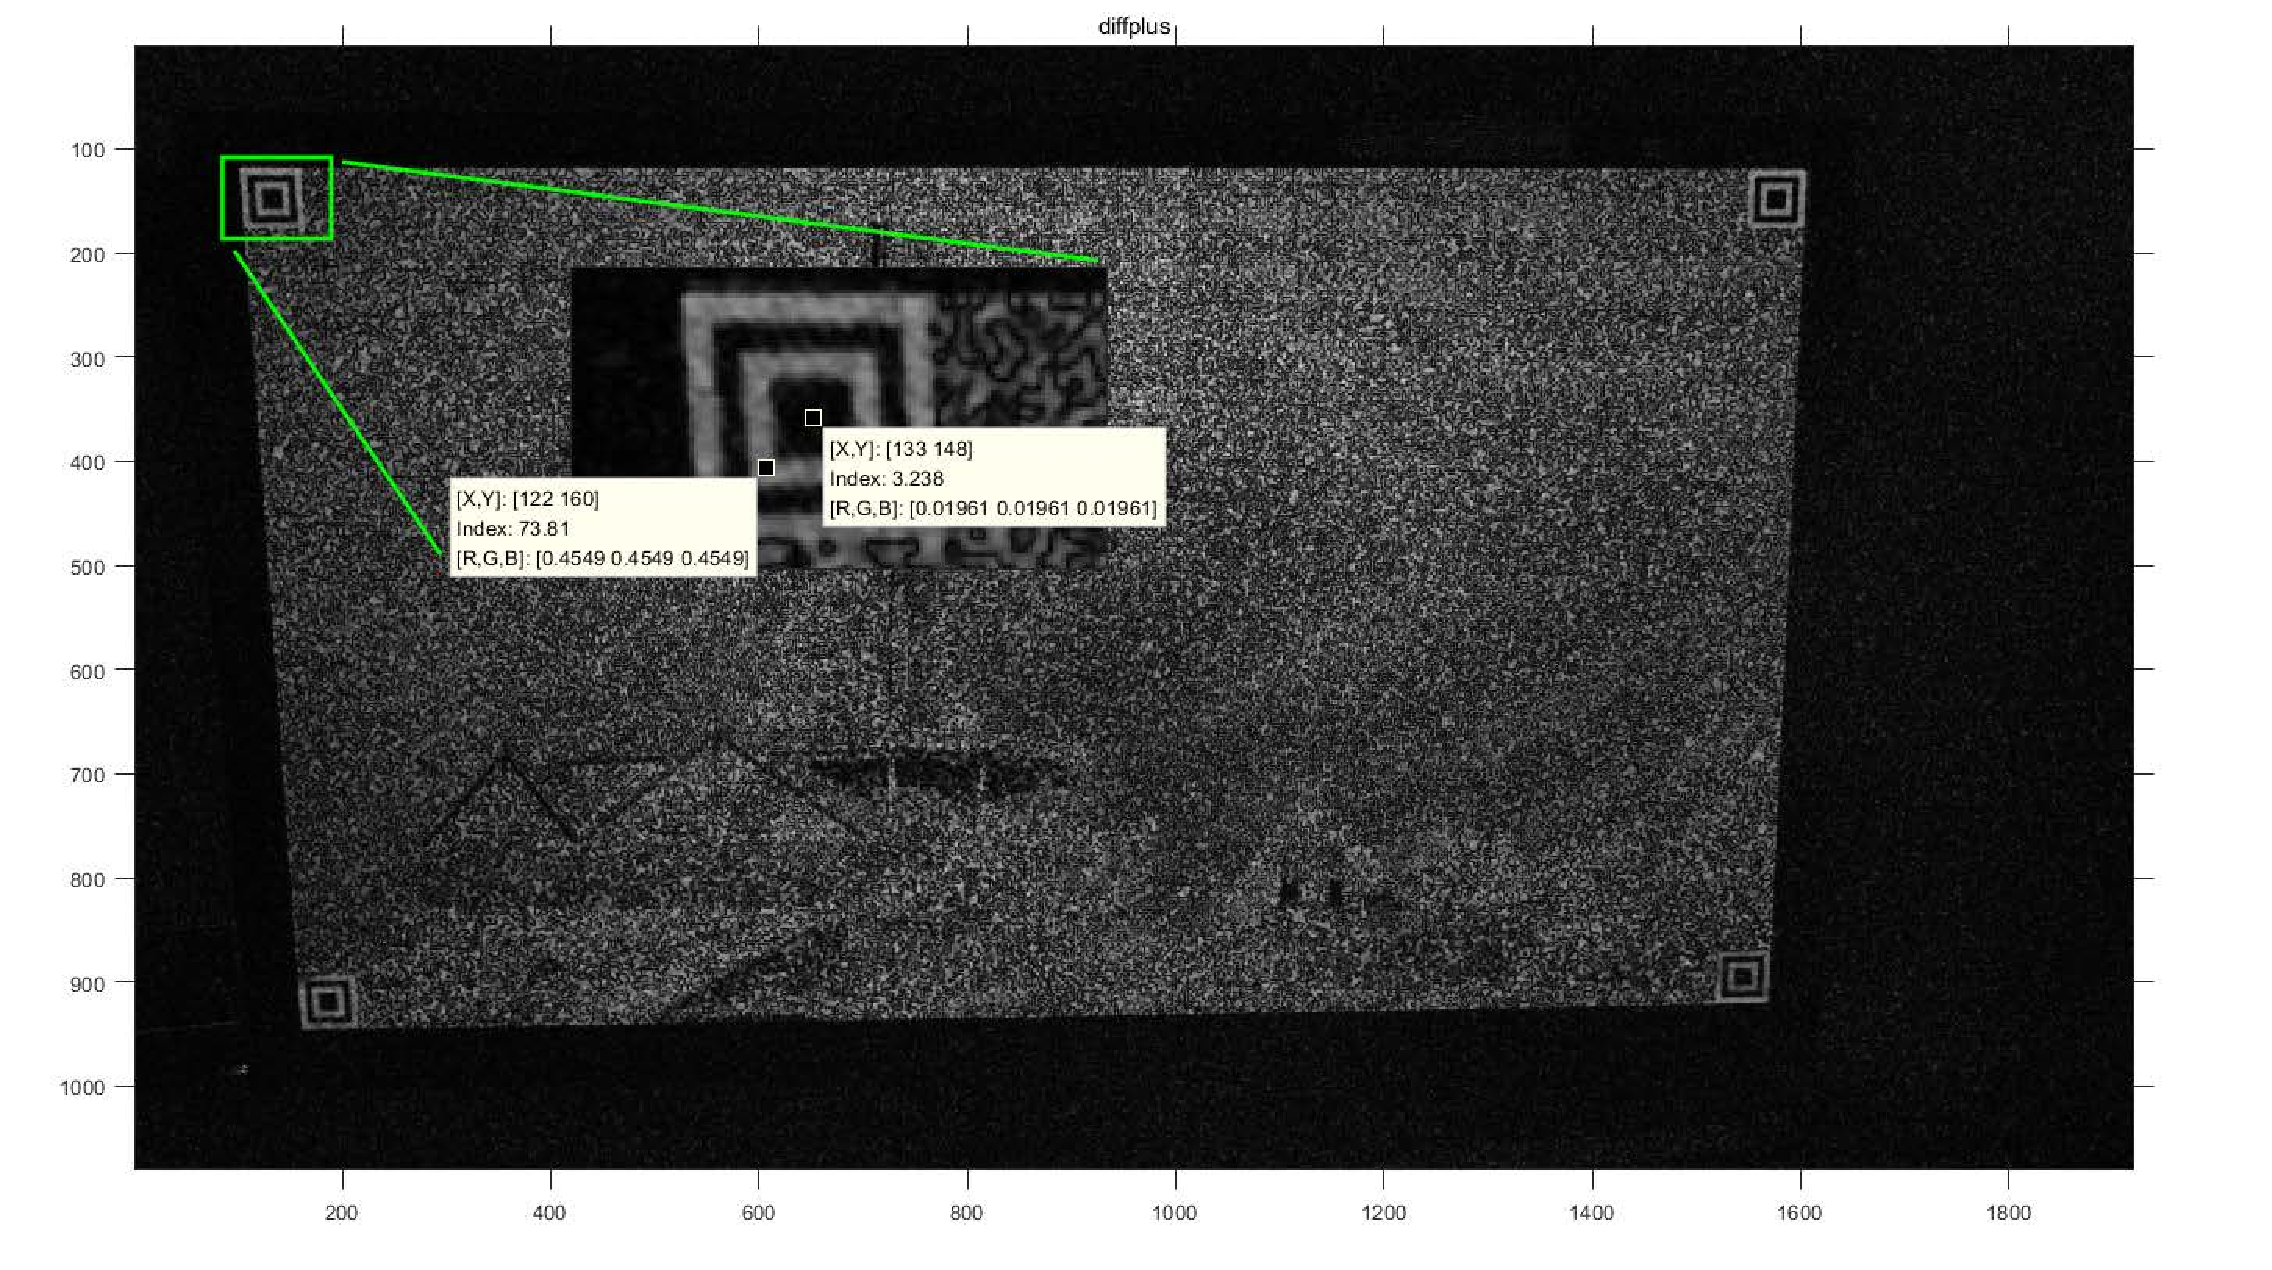
\includegraphics[width=1.0\textwidth]{images/5_Implementirung/nachdiff.pdf} 
\caption{Ein zu detektierendes Bild}
\label{fig:nachdiff}
\end{minipage}
\begin{minipage}[b]{0.49\textwidth} 
\centering 
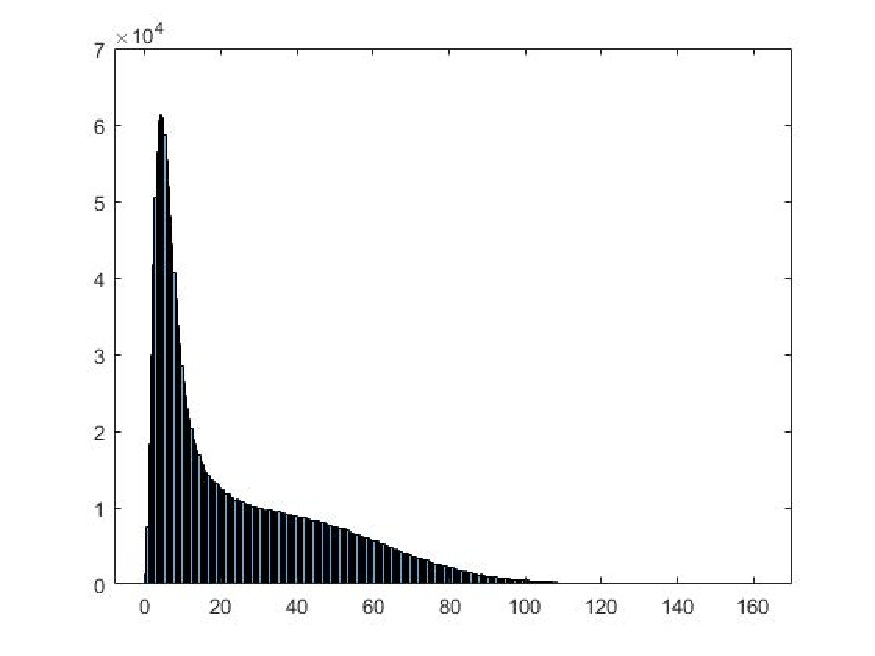
\includegraphics[width=0.8\textwidth]{images/5_Implementirung/histodiff.pdf}
\caption{Histogramm}
\label{fig:Histogramm}
\end{minipage}
\end{figure}

Anschließend wird dies Bild zu Bildverarbeitung Modul machen. Abbildung \ref{fig:binar} und Abbildung \ref{fig:morpho} zeigen die Ergebnis durch die Binarisierung bzw. die morphologische Operation.
Mit QR Muster Detektion kann die Zentrum des Muster bestimmen werden, wie in Abbildung \ref{fig:QR_muster} zeigt. Deshalb lassen sich der Modulationsbereich befinden. In Abbildung Abbildung\ref{fig:Mudulaition} wird es durch ein rotes Rechteck angezeigt. Schließlich mit eine projektive Transformation kann die Endergebnis erhalten, wie in Abbildung \ref{fig:Ergebnis1} gezeigt.

\begin{figure}[H]
\centering 
\begin{minipage}[b]{0.49\textwidth} 
\centering 
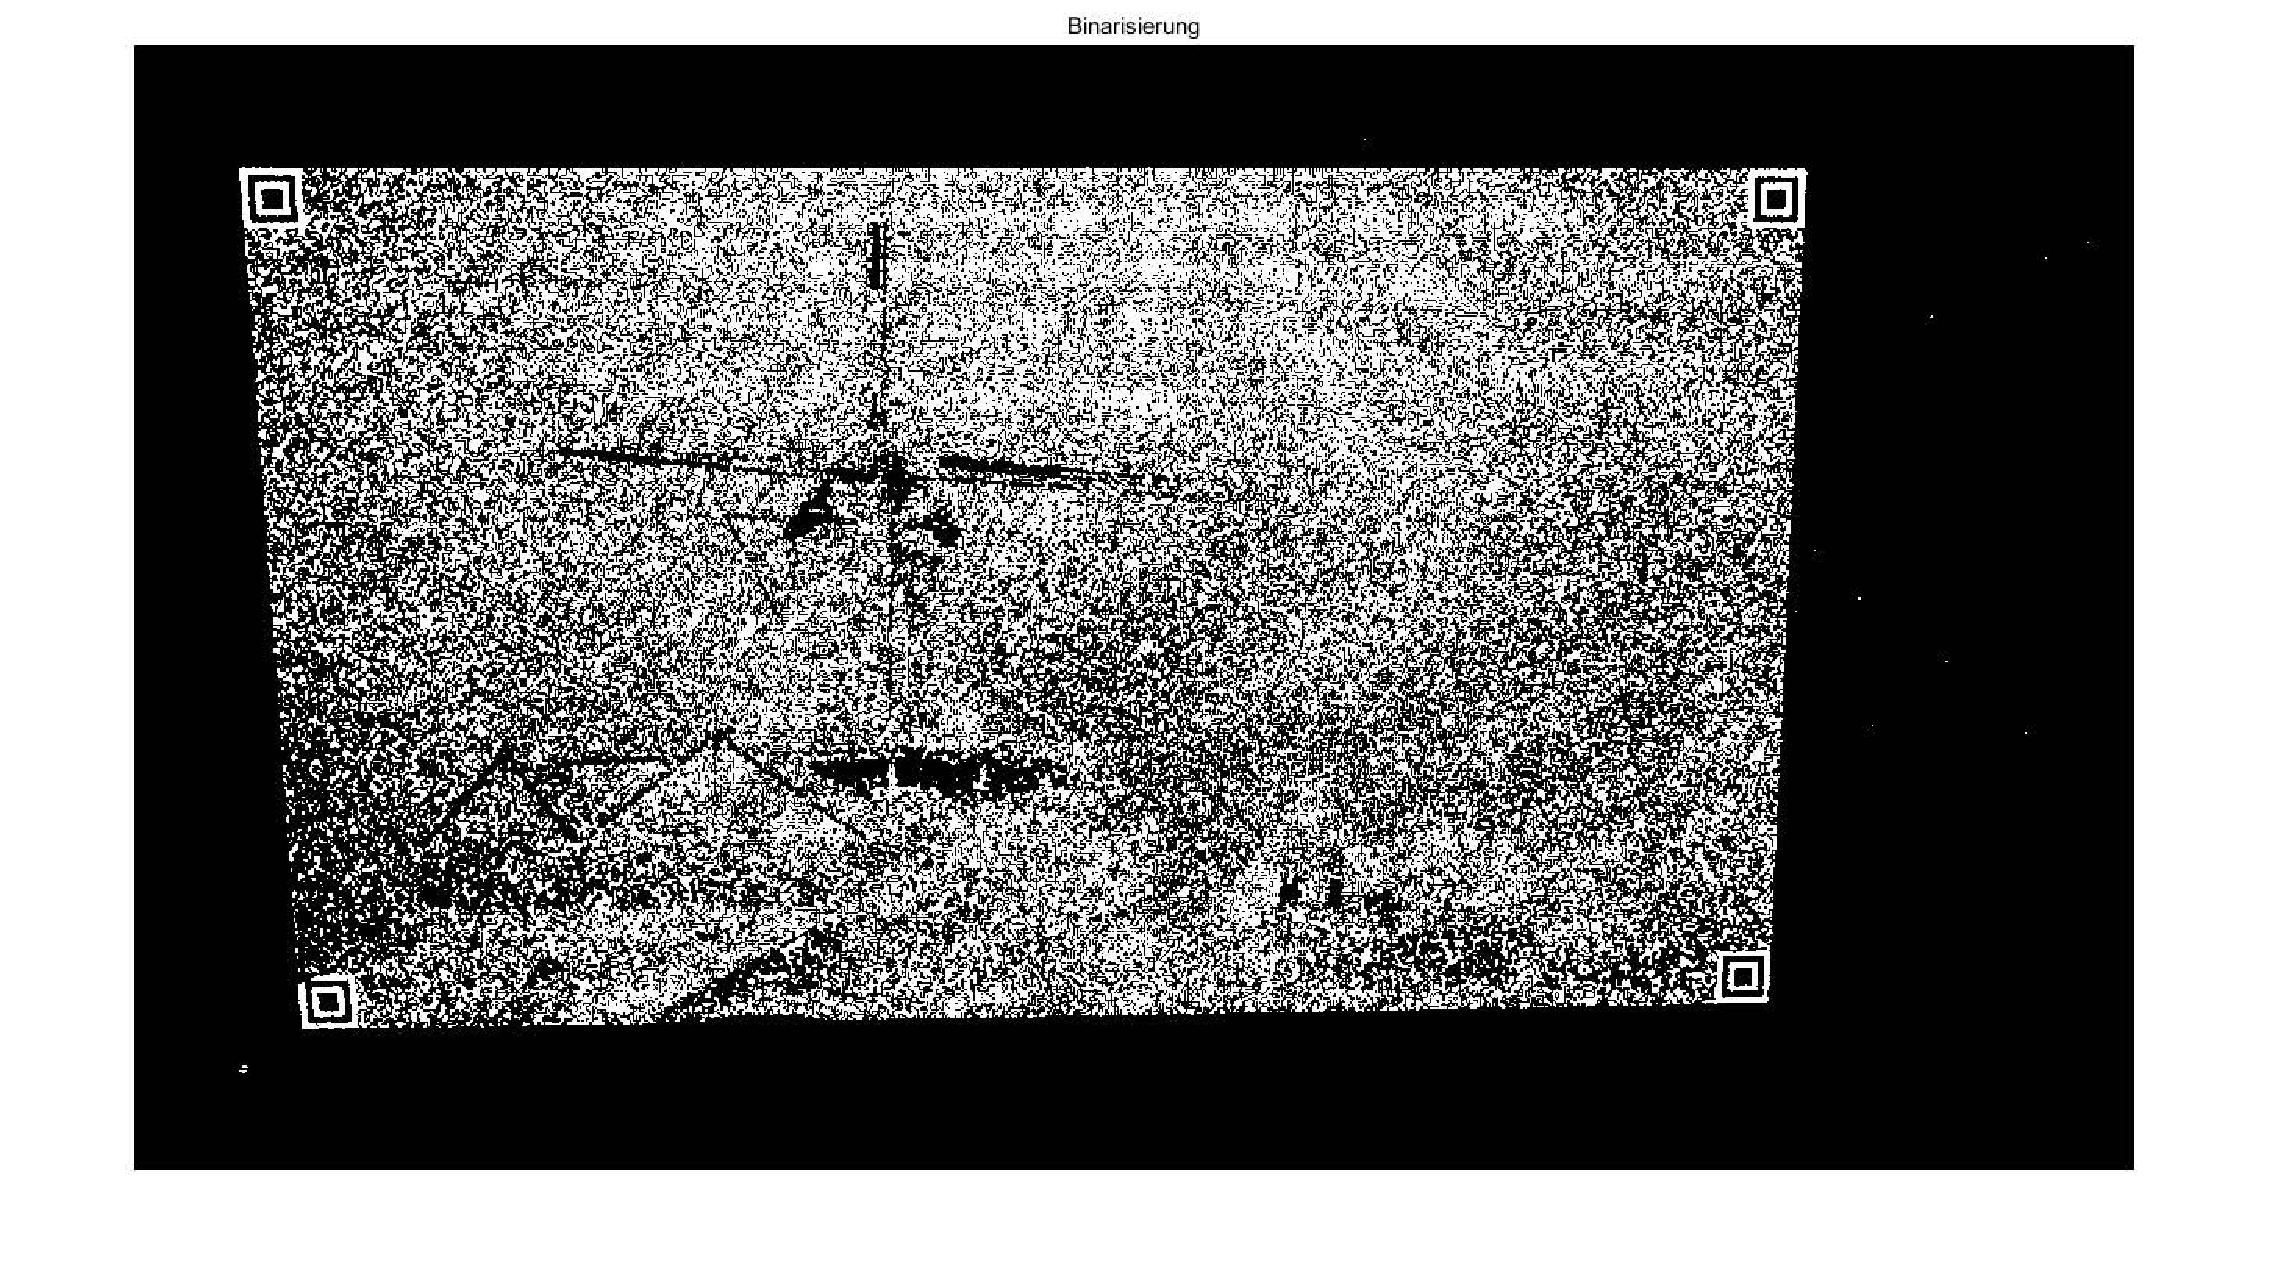
\includegraphics[width=1.0\textwidth]{images/5_Implementirung/Binar.pdf} 
\caption{Binär}
\label{fig:binar}
\end{minipage}
\begin{minipage}[b]{0.49\textwidth} 
\centering 
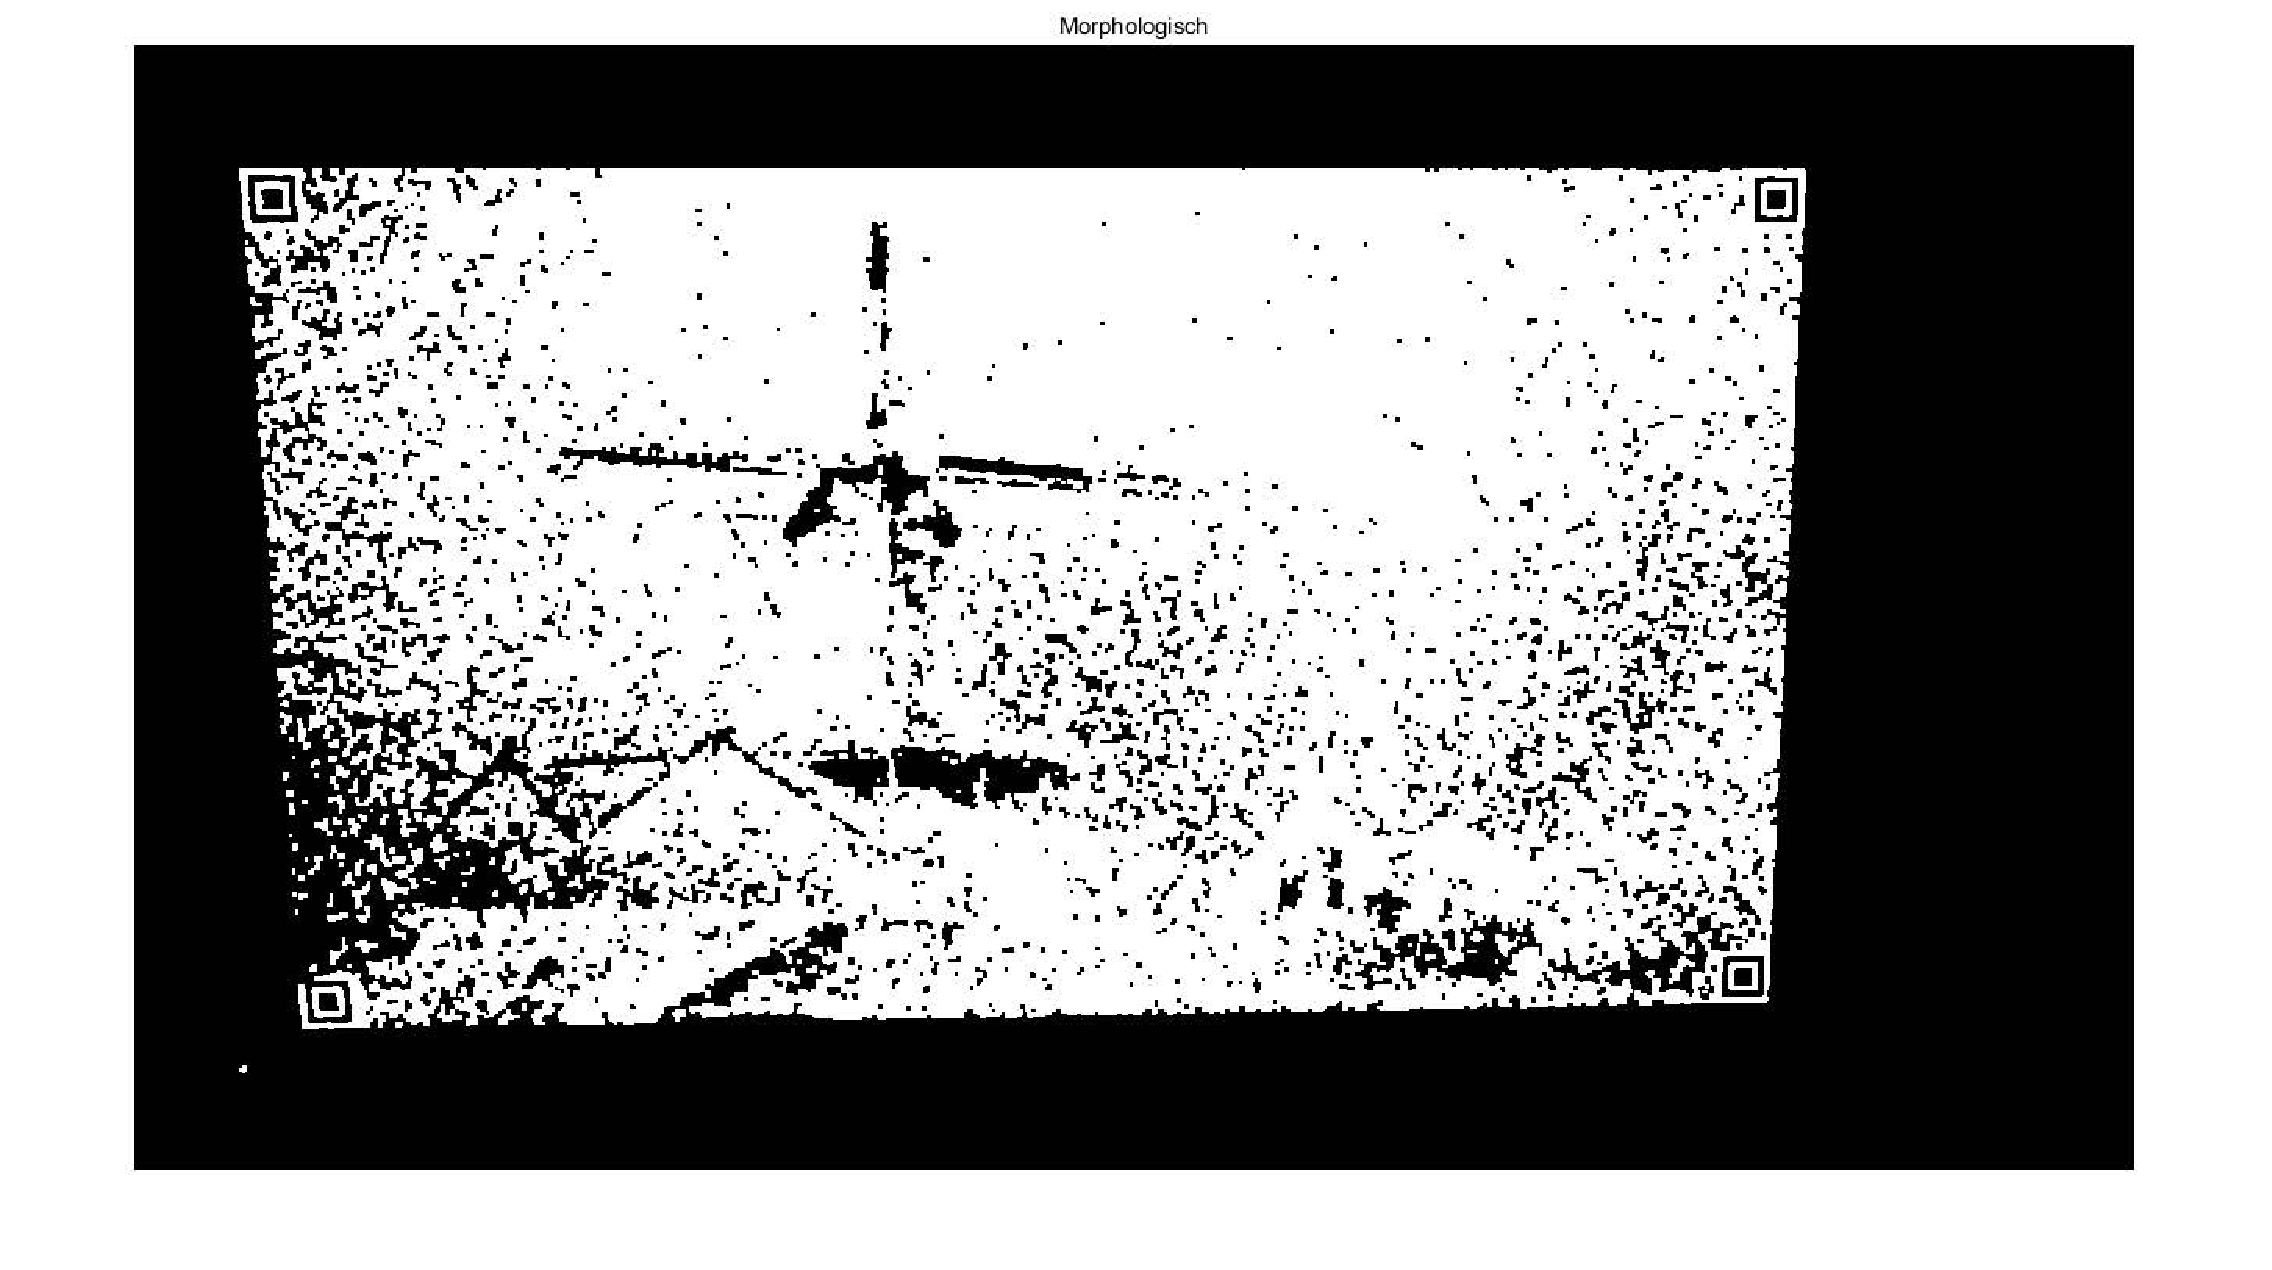
\includegraphics[width=1.0\textwidth]{images/5_Implementirung/morpho.pdf}
\caption{Morphologisch}
\label{fig:morpho}
\end{minipage}
\end{figure}

\begin{figure}[H]
\centering 
\begin{minipage}[b]{0.49\textwidth} 
\centering 
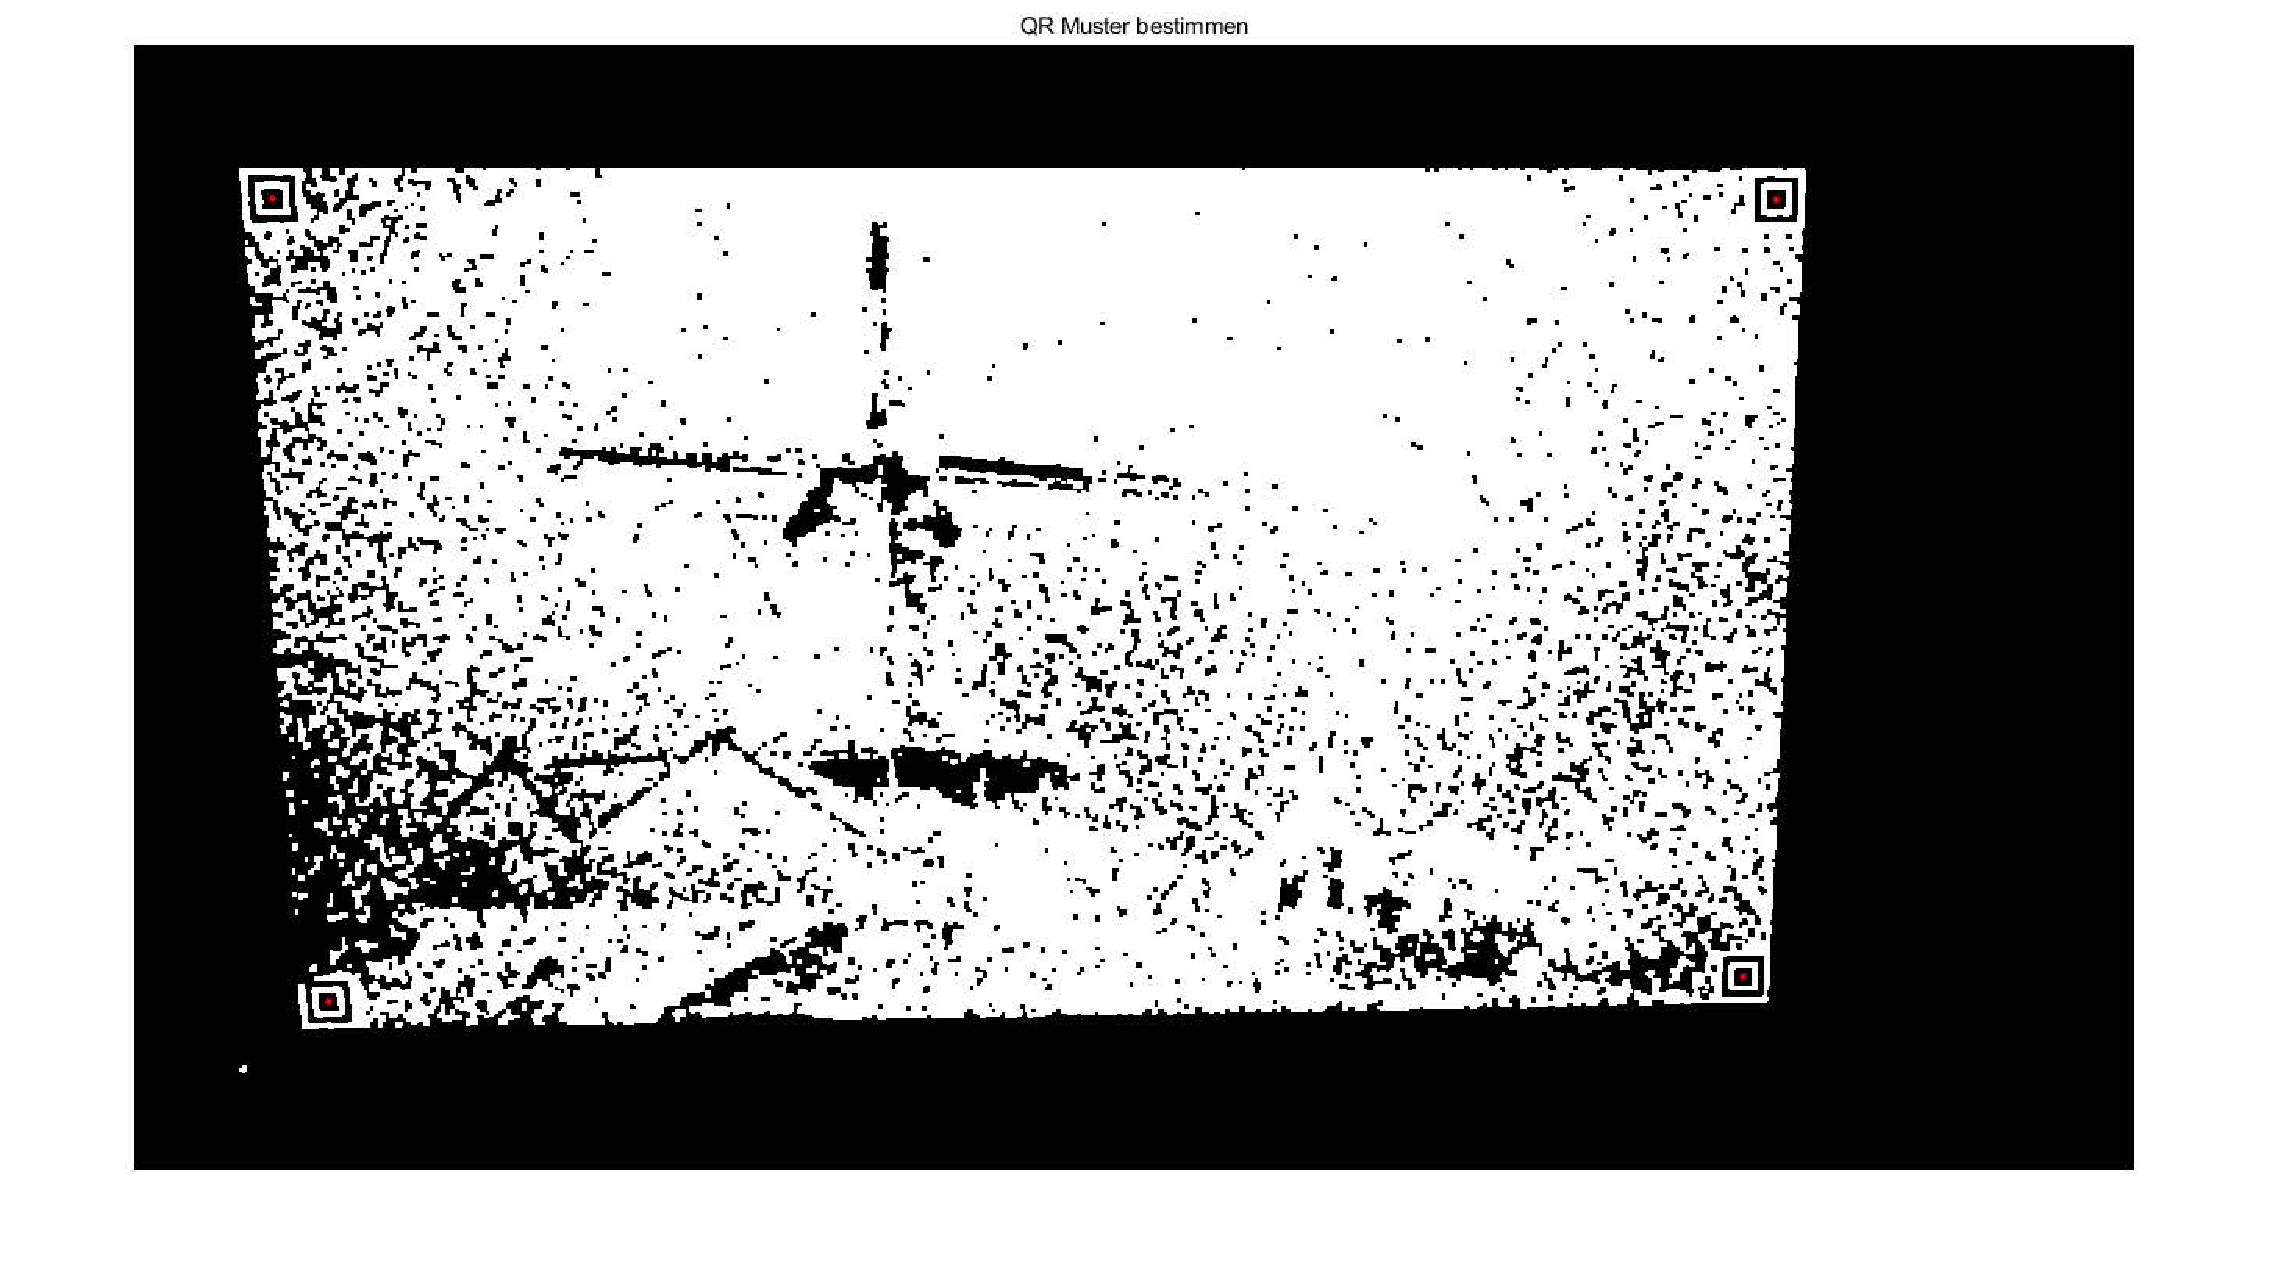
\includegraphics[width=1.0\textwidth]{images/5_Implementirung/QR_muster.pdf} 
\caption{QR Muster}
\label{fig:QR_muster}
\end{minipage}
\begin{minipage}[b]{0.49\textwidth} 
\centering 
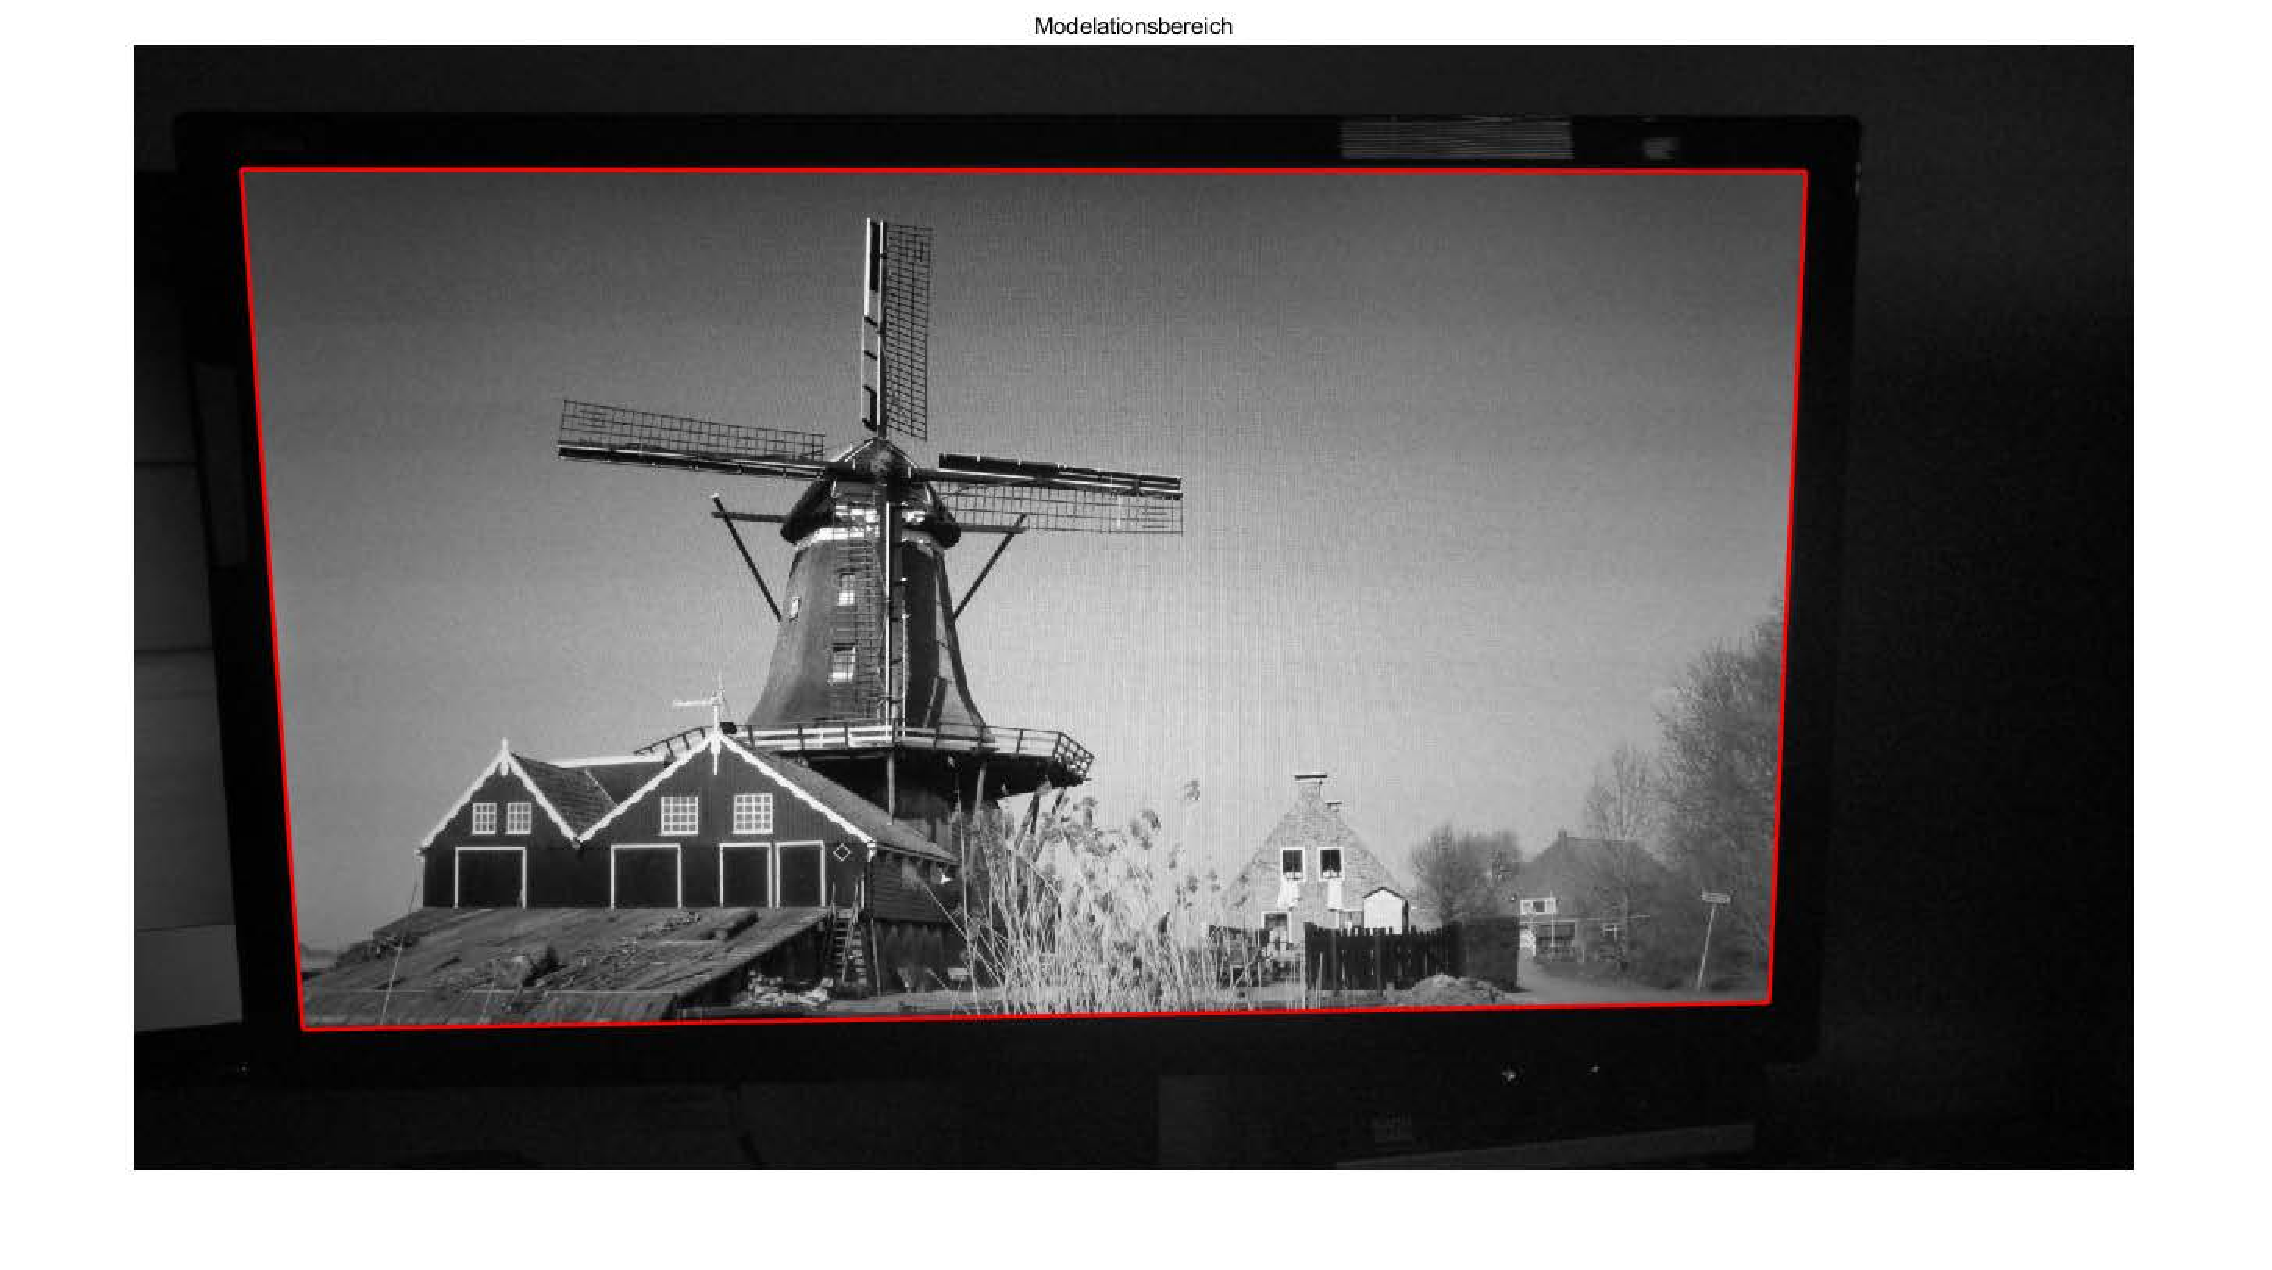
\includegraphics[width=1.0\textwidth]{images/5_Implementirung/Mudulaition.pdf}
\caption{Mudulaitionbereich}
\label{fig:Mudulaitionbereich}
\end{minipage}
\end{figure}

\begin{figure}[H]
 \centering 
  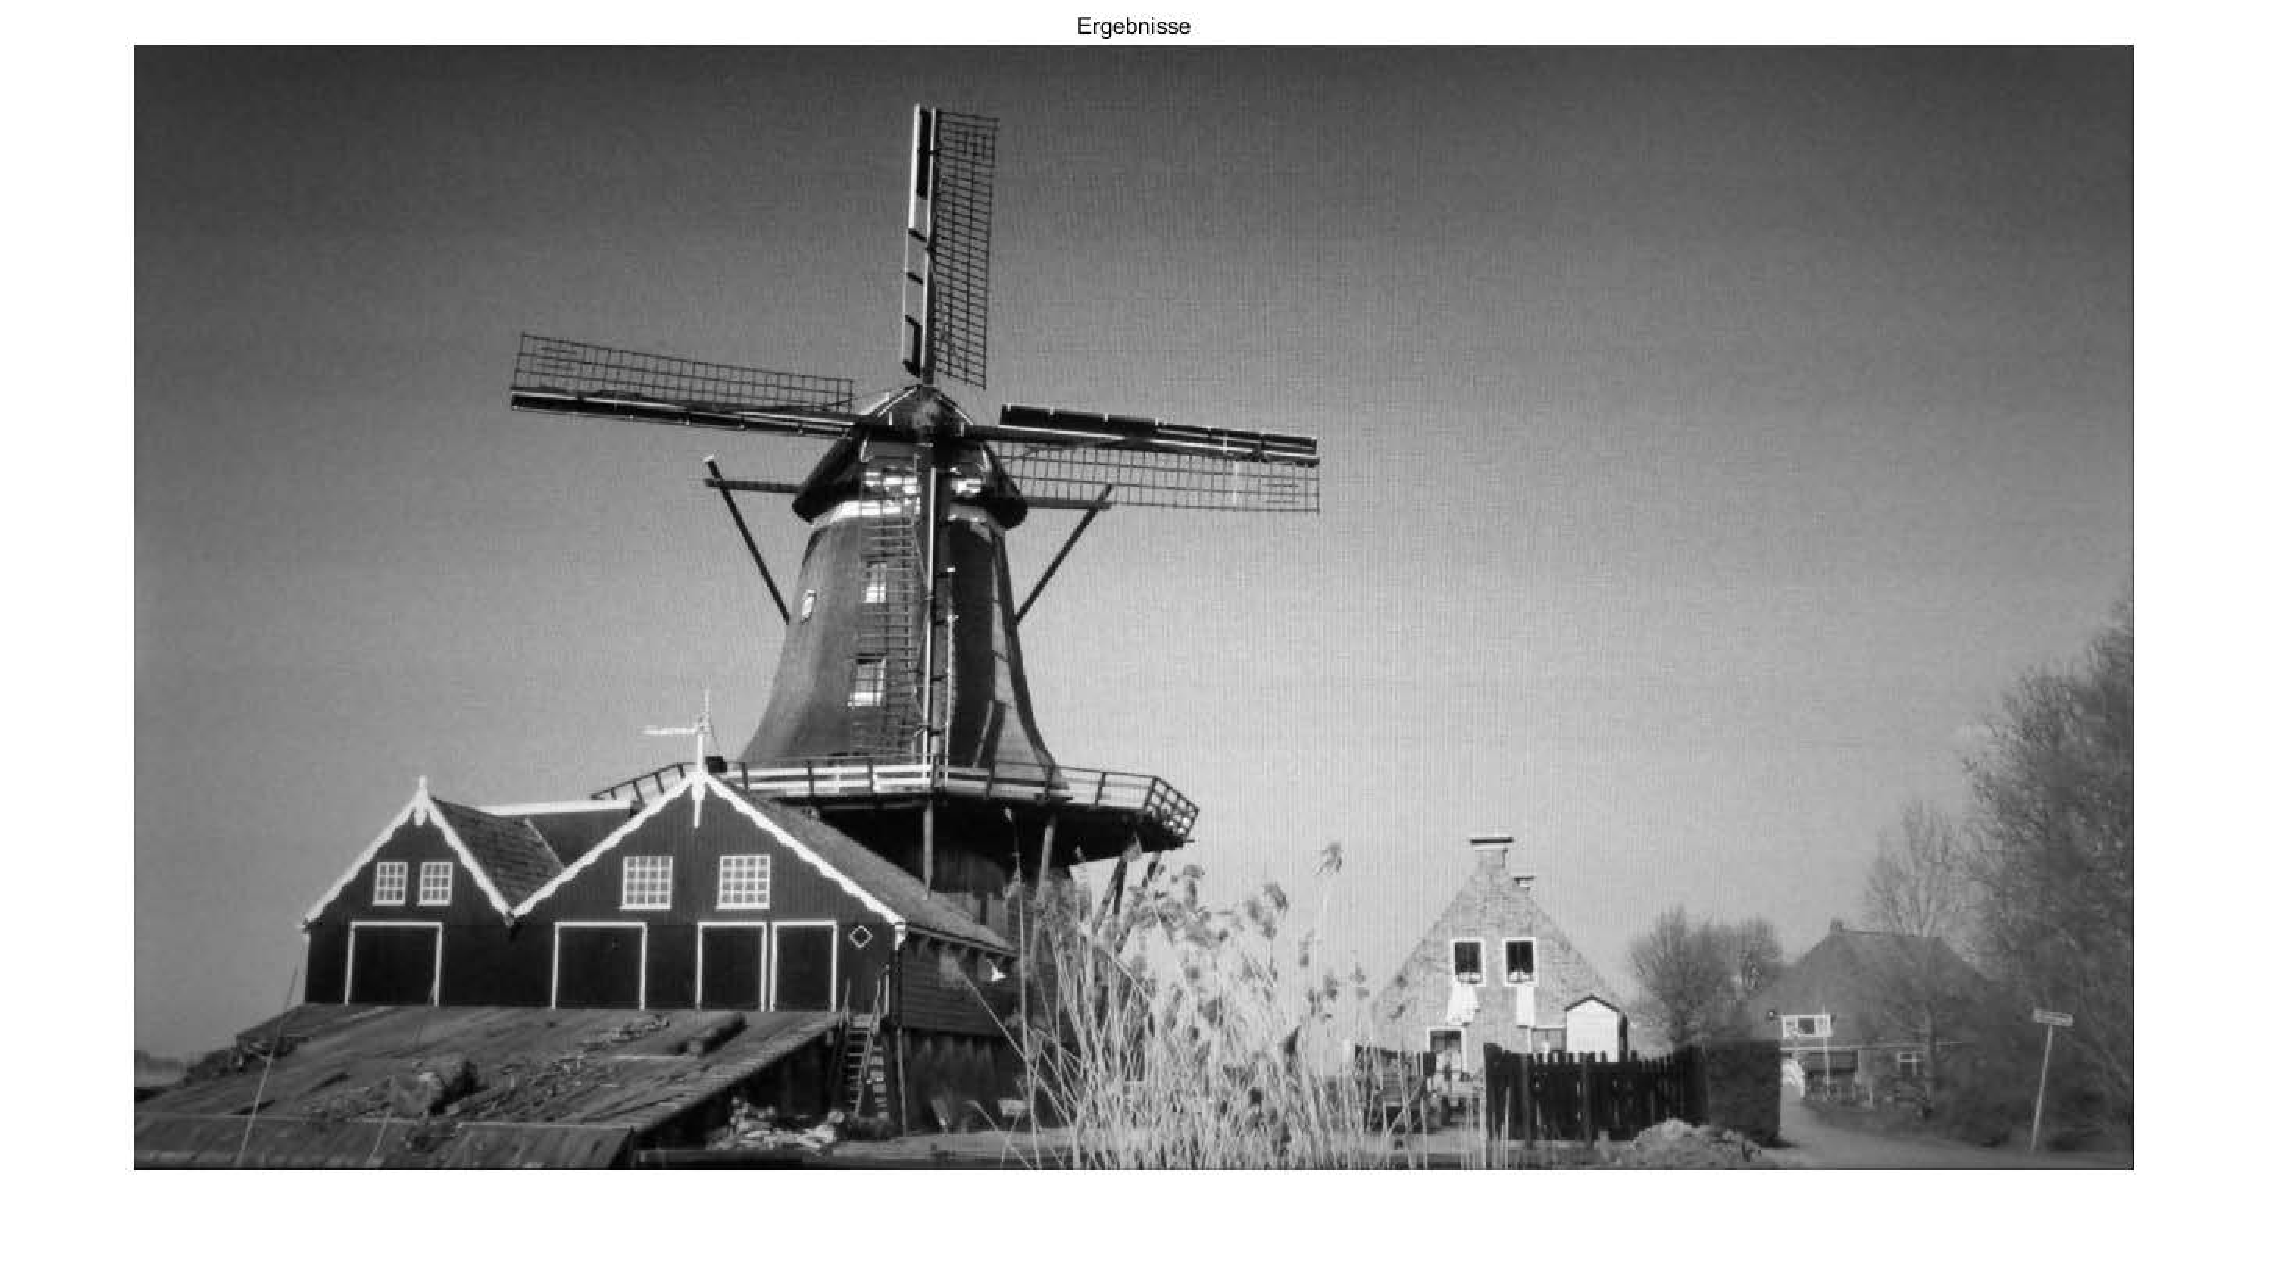
\includegraphics[keepaspectratio,width=1.0\textwidth]{images/5_Implementirung/ergeb.pdf}
 \caption{Ergebnis der 1. Methode}
 \label{fig:Ergebnis1}
\end{figure}

Als Nächst einige Ergebnisse der Verwendungen von die 1. Methode wird angegeben.

Bilder


\section{Implementierung der zweiten Verfahren}

Hier wird der Implementierung für zweite Methode vorstellen. Das Bild stammt aus einer Reihe von achten Bildern, die durch Google Pixel mit Stativ aufgenommen wurden. Deswegen wird hier Bildregistration nicht verwendet. Dies bedeutet, dass sich der Inhalt des Videos verändern lassen. Die Modulationsamplitude werden als 6 erstellt, anschließend Daten Datenblock als $ 4 \times 4 Pixel$. 

Durch das Wissen des 4. Kapitels, wird von diese Bildern eine Reihe Differenzbilder enthalten. 3 mit größte $``Energie"$ Differenzbilder werden addiert, um ein zu detektierendes Bild zu entstehen, wie in Abbildung \ref{fig:diff2} gezeigt. Anschließend mit Verwendung der Binarisierungsmethod, hier lauft Ostu Schwellen methode, wird ein Binärbild bekommen, indem der Modulationsbereich von Bild herausgezogen wird. Um die kleinen Punkte und Lücken zu beseitigen, lassen sich eine morphologische Operation durchführen. Das hier benutzte Strukturelement ist ein $5 \times 5$ Quadrat. 
Diese Effekt der beider Operationen werden in Abbildung \ref{fig:binar2} und Abbildung \ref{fig:morph2} gezeigt. Danach um die Einfluss der Kamera-Verzerrung zu verhindern, wird die Binärbild mit eine Cross Dilatation machen, also $ n_{around} = 1$. Das Struktur der Cross Dilatation wird in Abbildung gezeigt und Abbildung \ref{fig:cd} zeigt diese Operation. Schließlich lassen das Bildzentrum auf den Ursprung setzen , und durch Vergleich der Integralwerte kann die längste Linien, die oben, unten, links und rechts legt, gefunden werden. Außerdem um die Berechnungskosten zu reduzieren, werden die Linien innerhalb von $ \pm 10^{\circ} $ erkannt. 




\begin{figure}[H]
\centering 
\begin{minipage}[b]{0.49\textwidth} 
\centering 
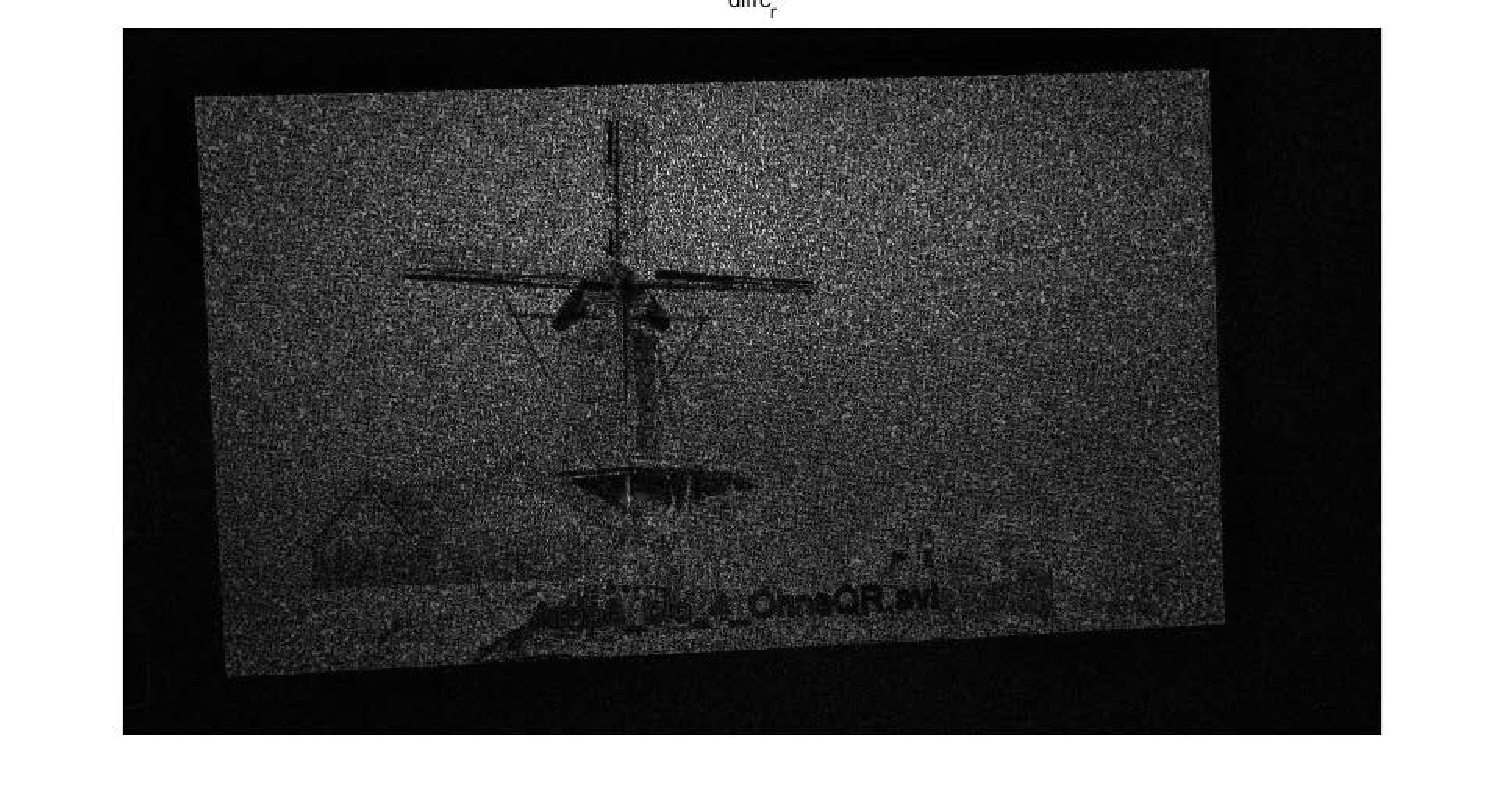
\includegraphics[width=1.0\textwidth]{images/5_Implementirung/2/diff.pdf} 
\caption{Ein zu detektierendes Bild}
\label{fig:diff2}
\end{minipage}
\begin{minipage}[b]{0.49\textwidth} 
\centering 
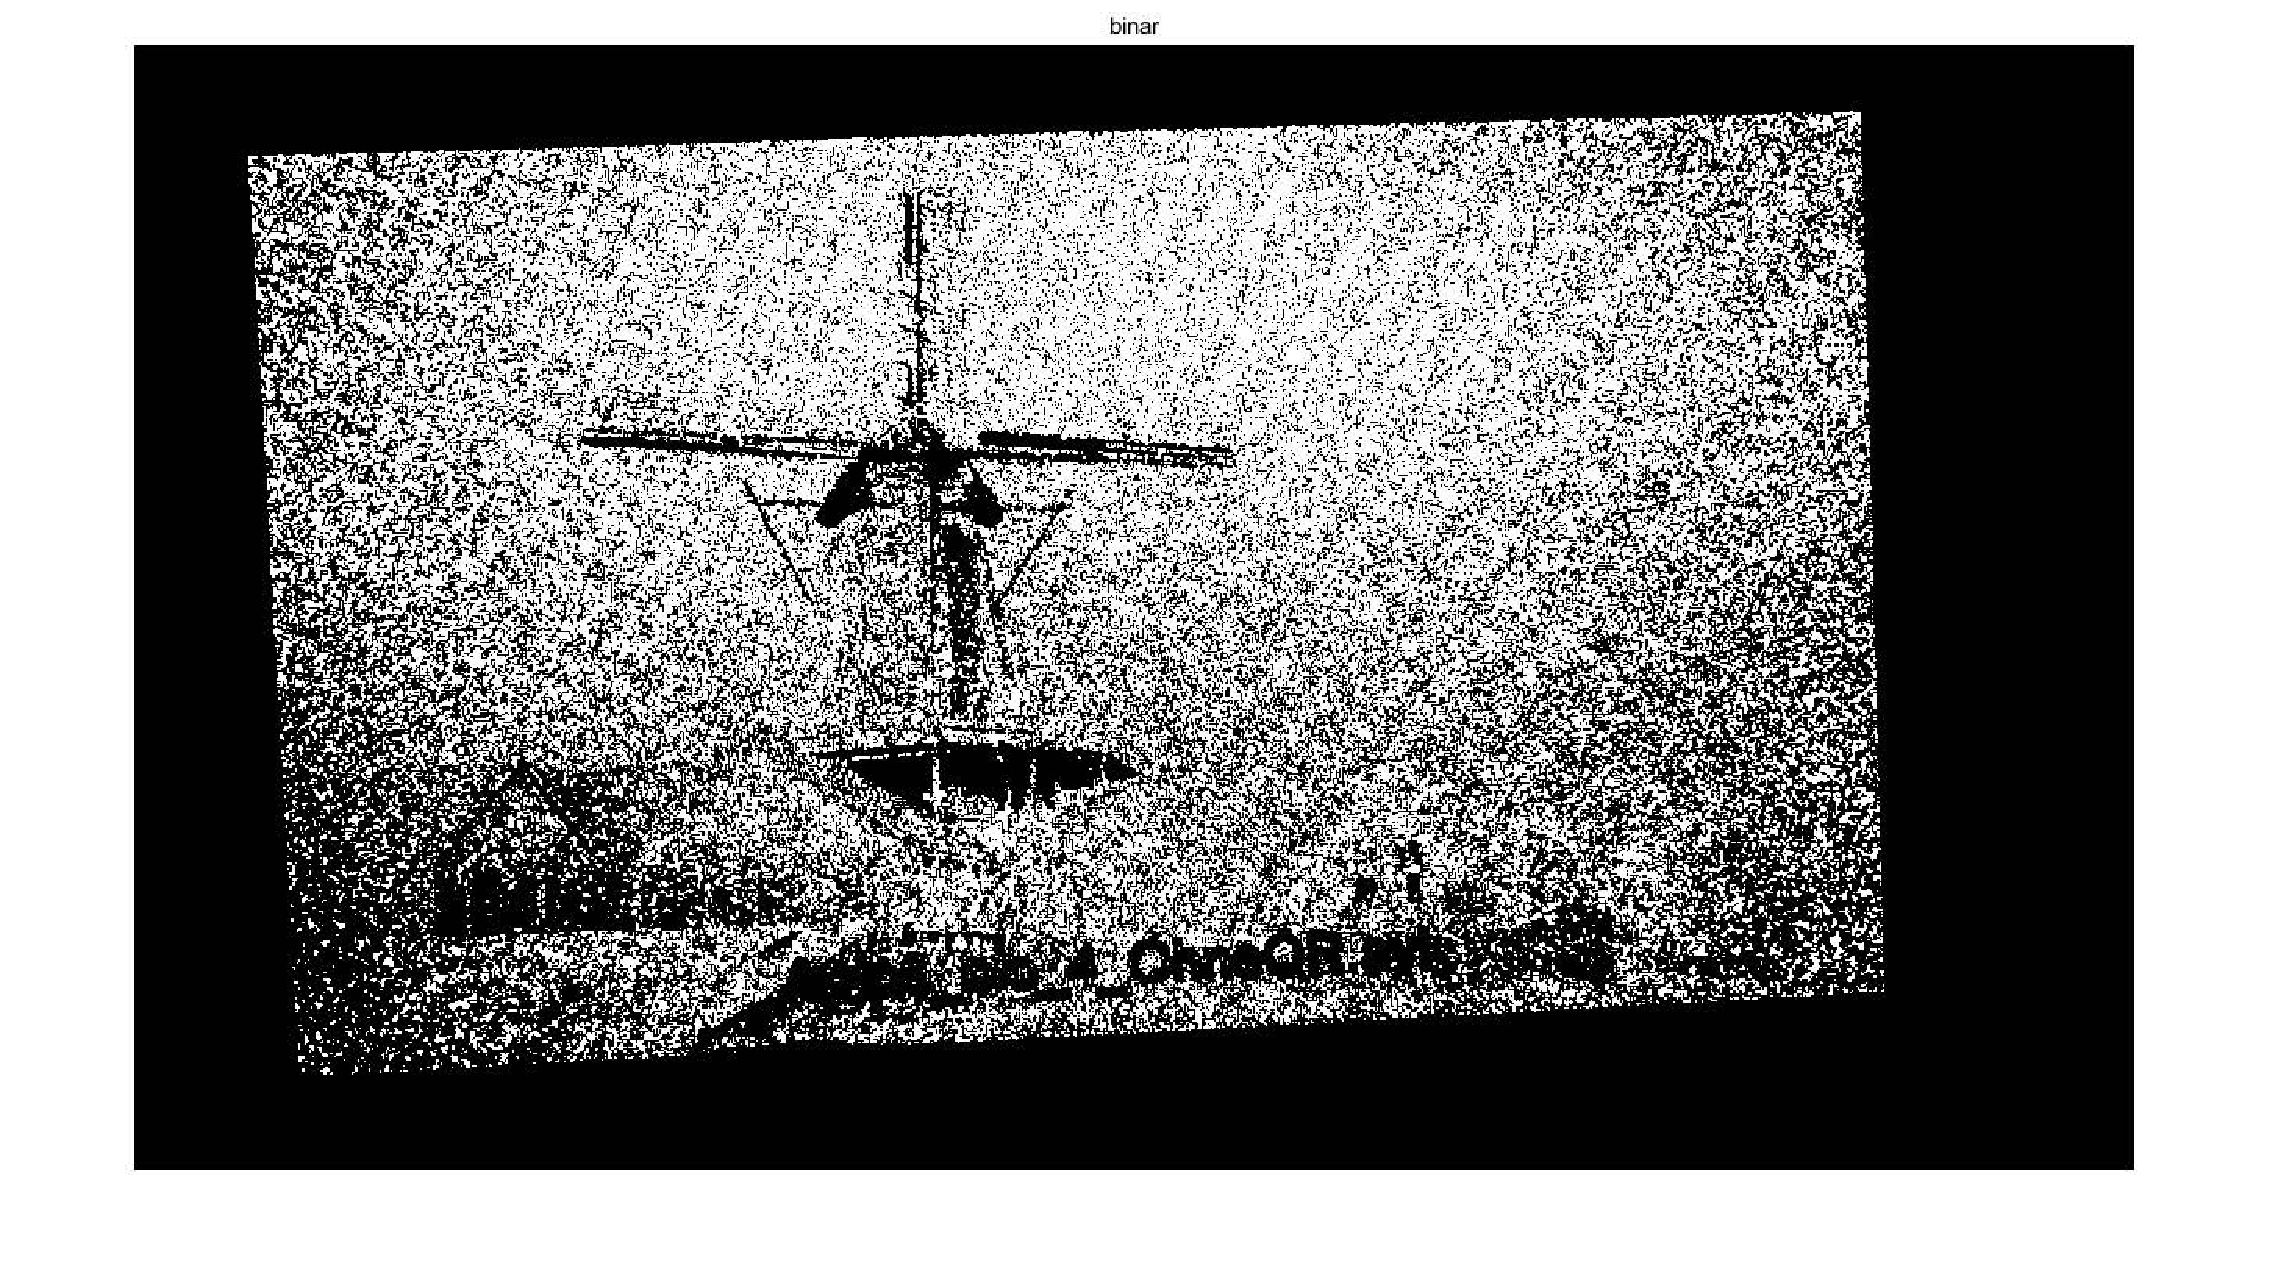
\includegraphics[width=1.0\textwidth]{images/5_Implementirung/2/bina.pdf}
\caption{Binarisierung}
\label{fig:binar2}
\end{minipage}
\end{figure}

\begin{figure}[H]
\centering 
\begin{minipage}[b]{0.49\textwidth} 
\centering 
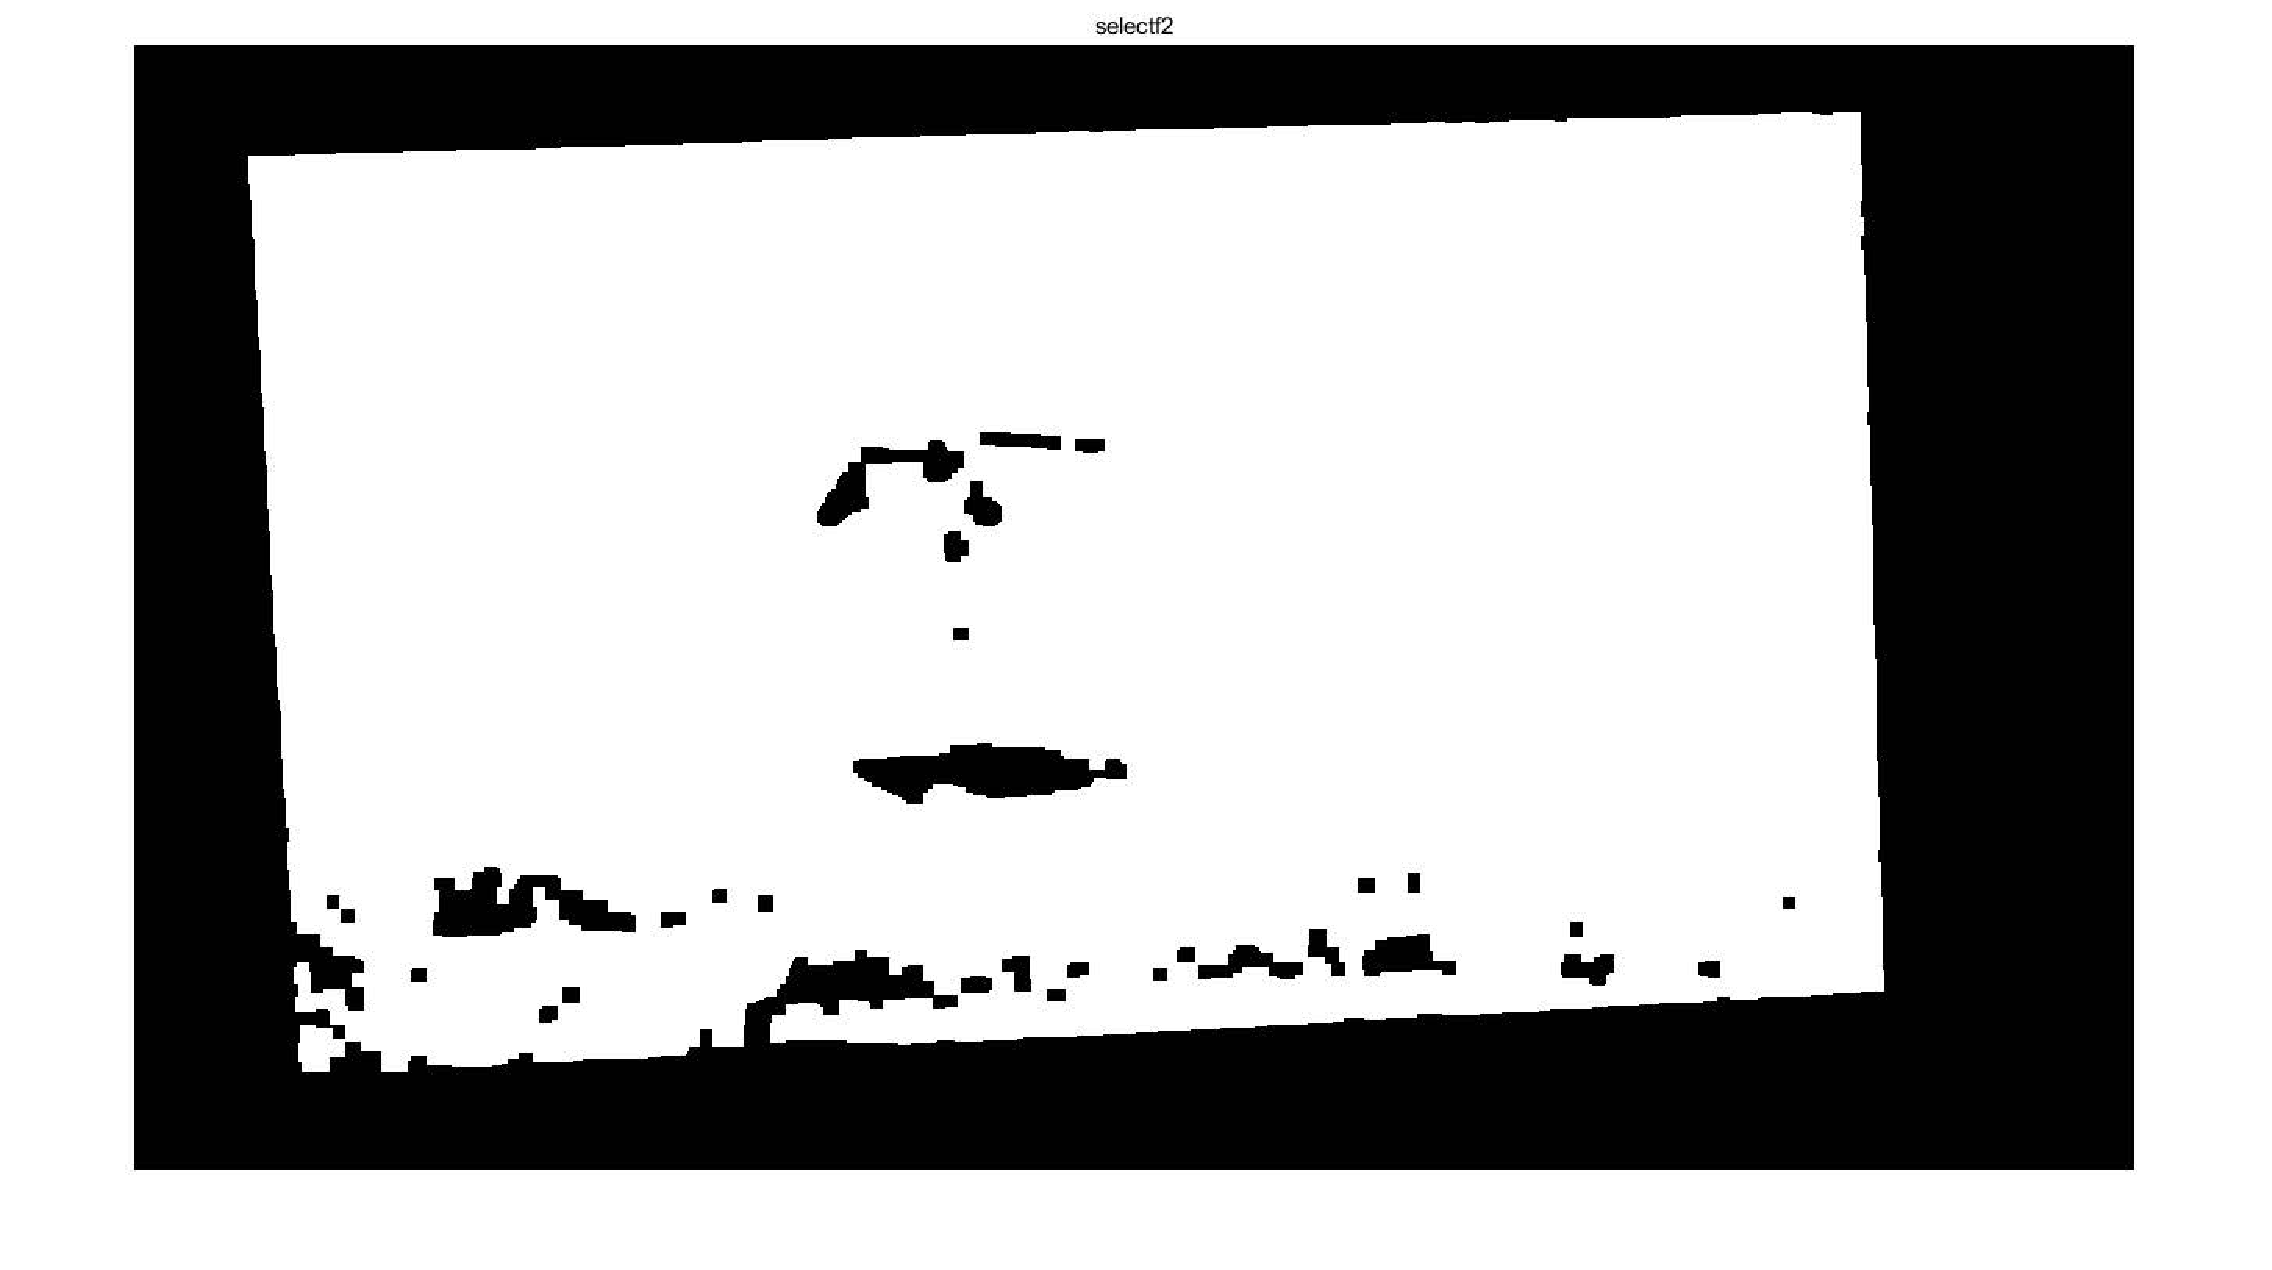
\includegraphics[width=1.0\textwidth]{images/5_Implementirung/2/morpho.pdf} 
\caption{Morphologisch}
\label{fig:morph2}
\end{minipage}
\begin{minipage}[b]{0.49\textwidth} 
\centering 
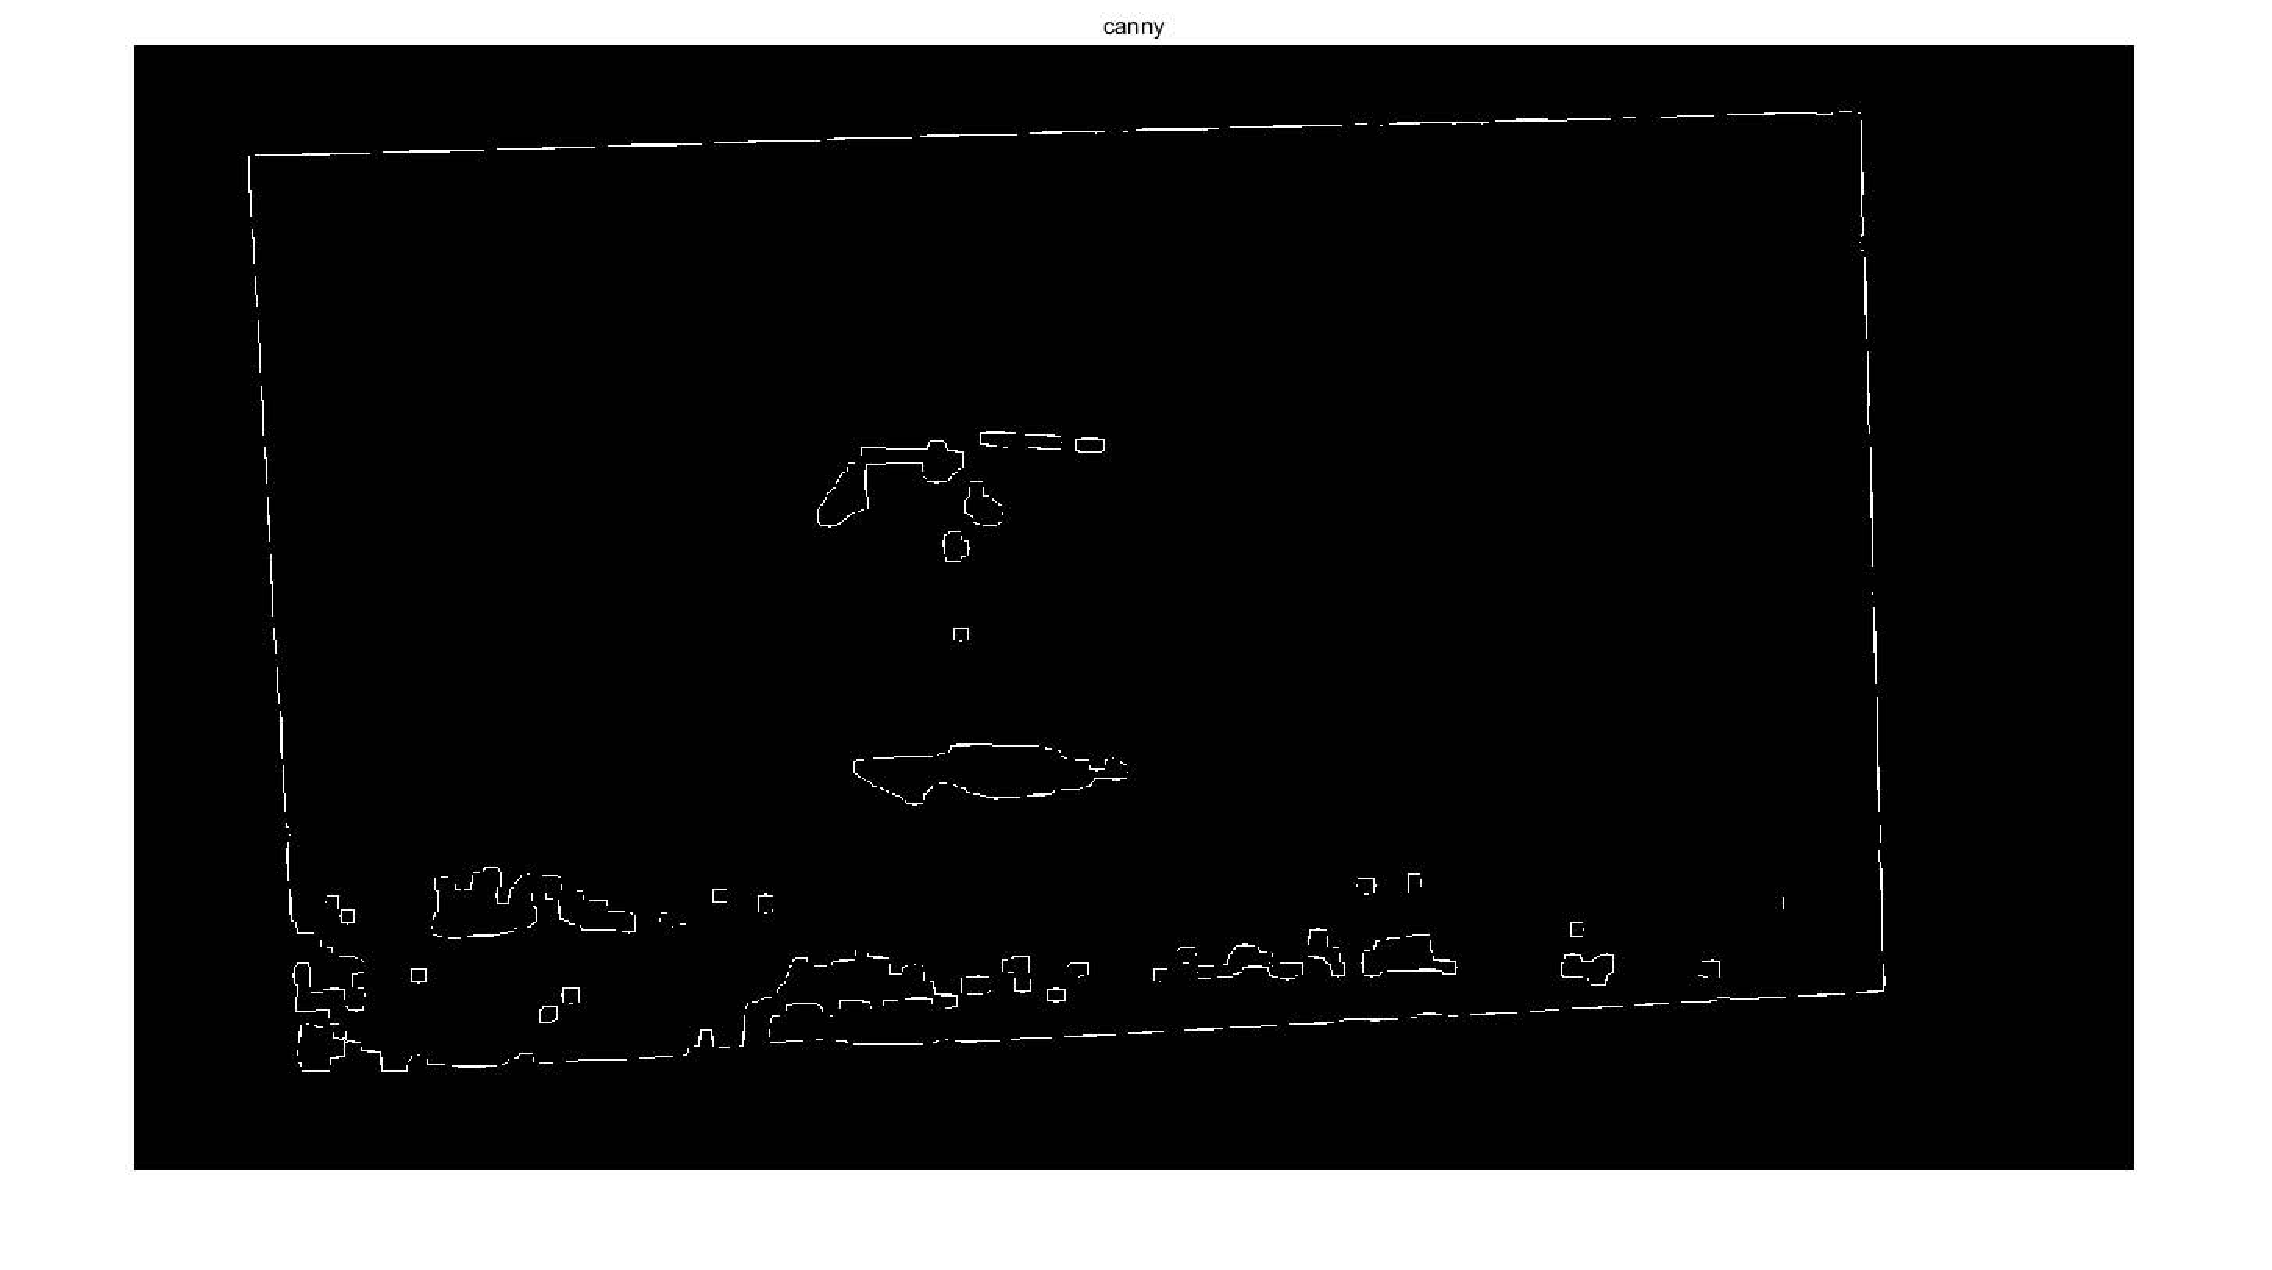
\includegraphics[width=1.0\textwidth]{images/5_Implementirung/2/canny.pdf}
\caption{Canny Detektion}
\label{fig:canny}
\end{minipage}
\end{figure}

\begin{figure}[H]
\centering 
\begin{minipage}[b]{0.49\textwidth} 
\centering 
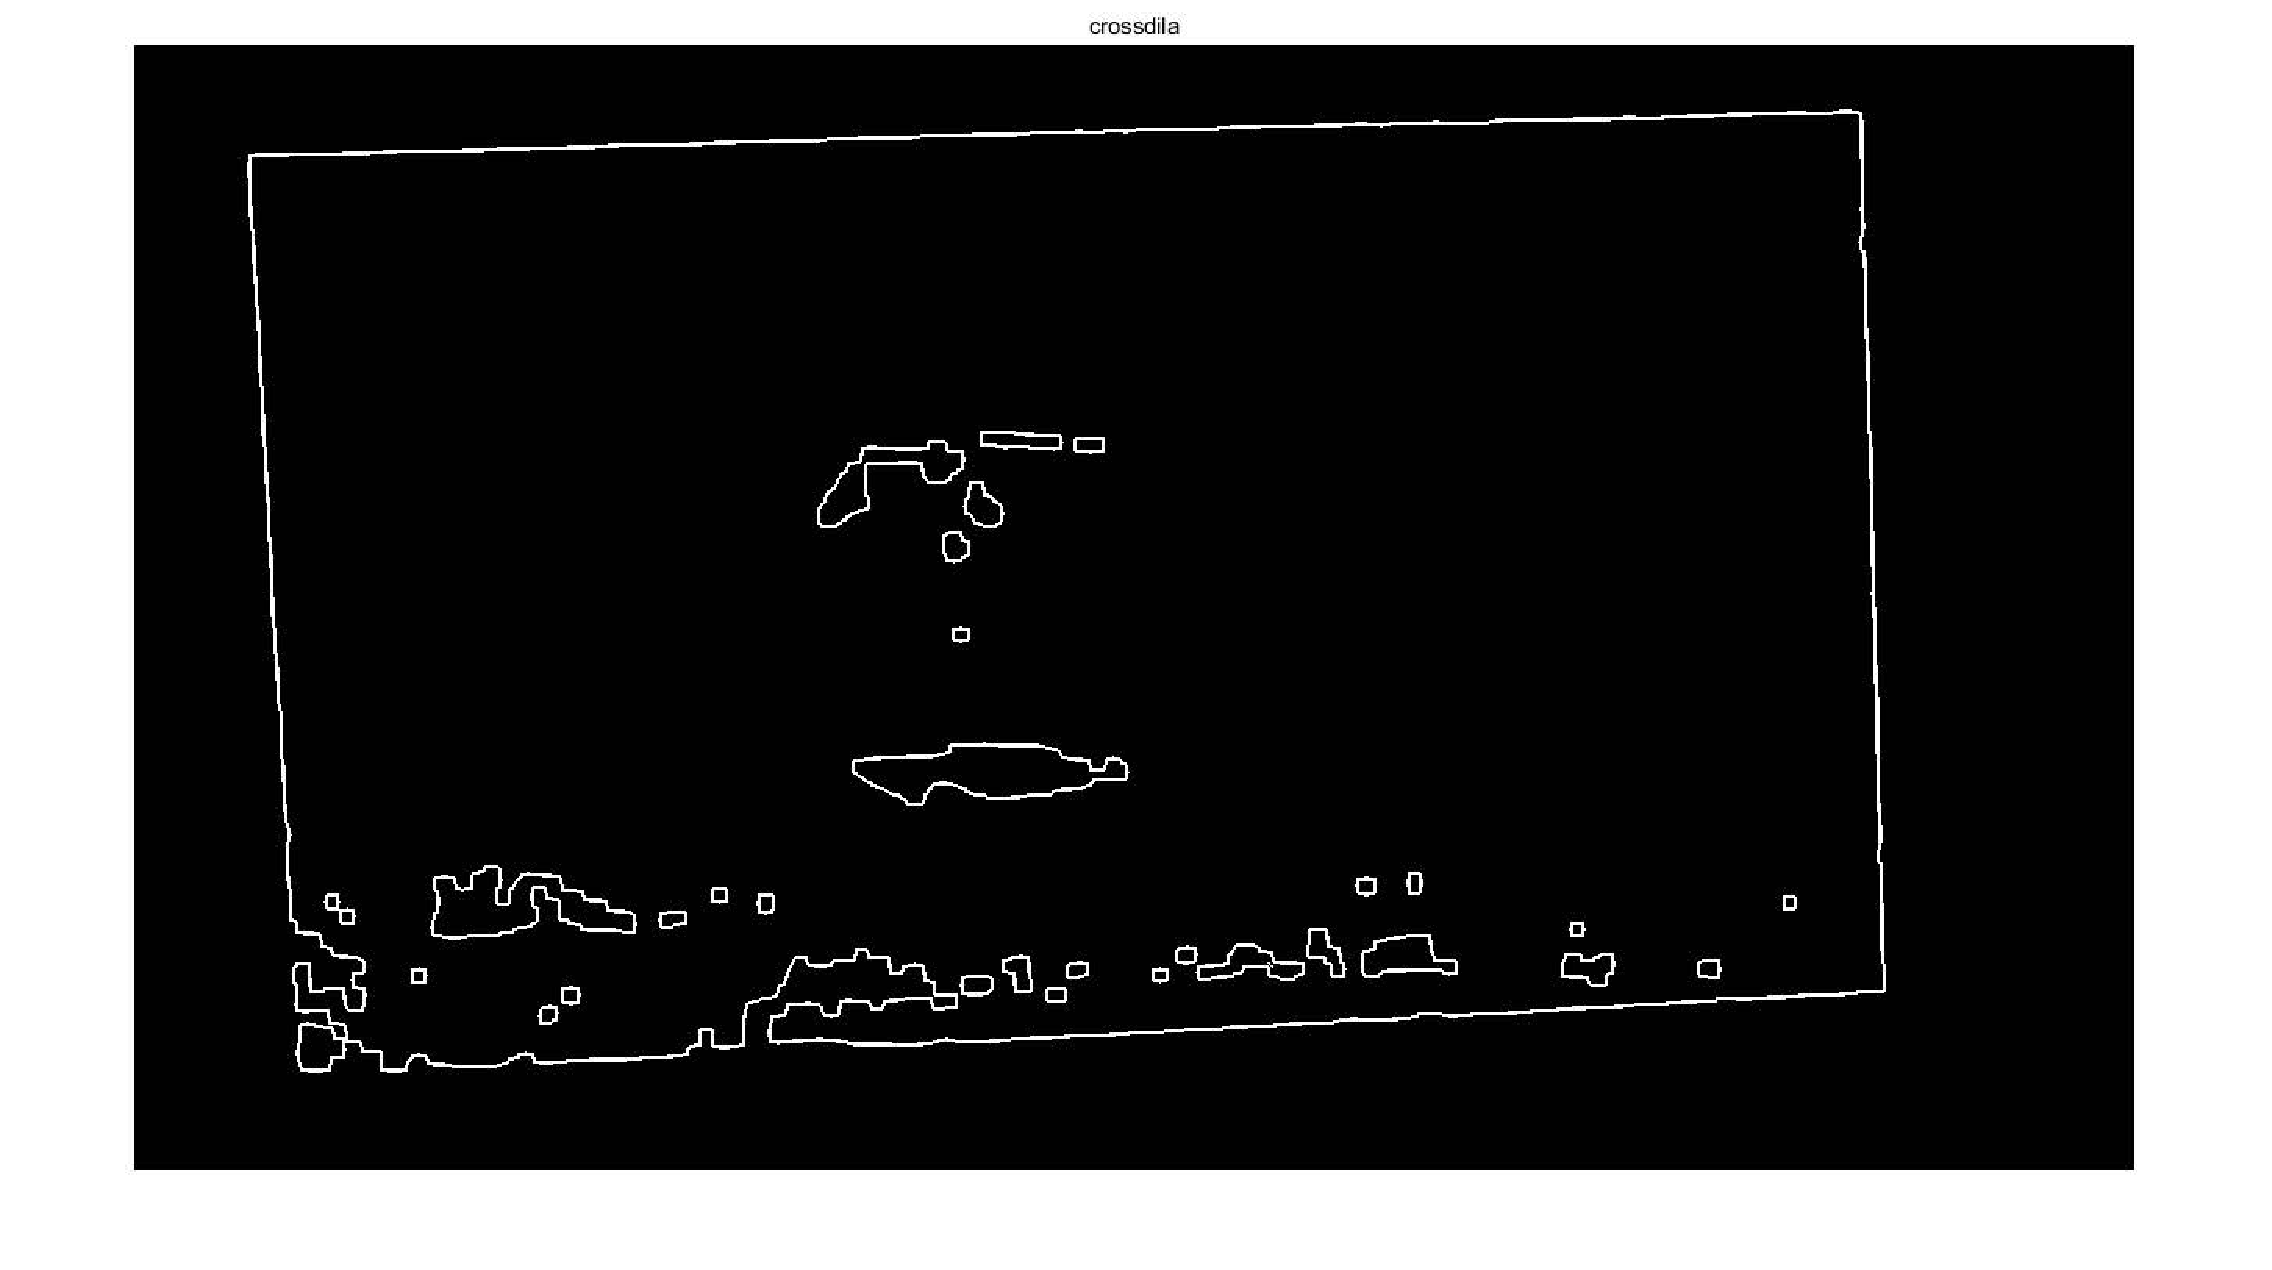
\includegraphics[width=1.0\textwidth]{images/5_Implementirung/2/cd.pdf} 
\caption{Cross Dilatation}
\label{fig:cd}
\end{minipage}
\begin{minipage}[b]{0.49\textwidth} 
\centering 
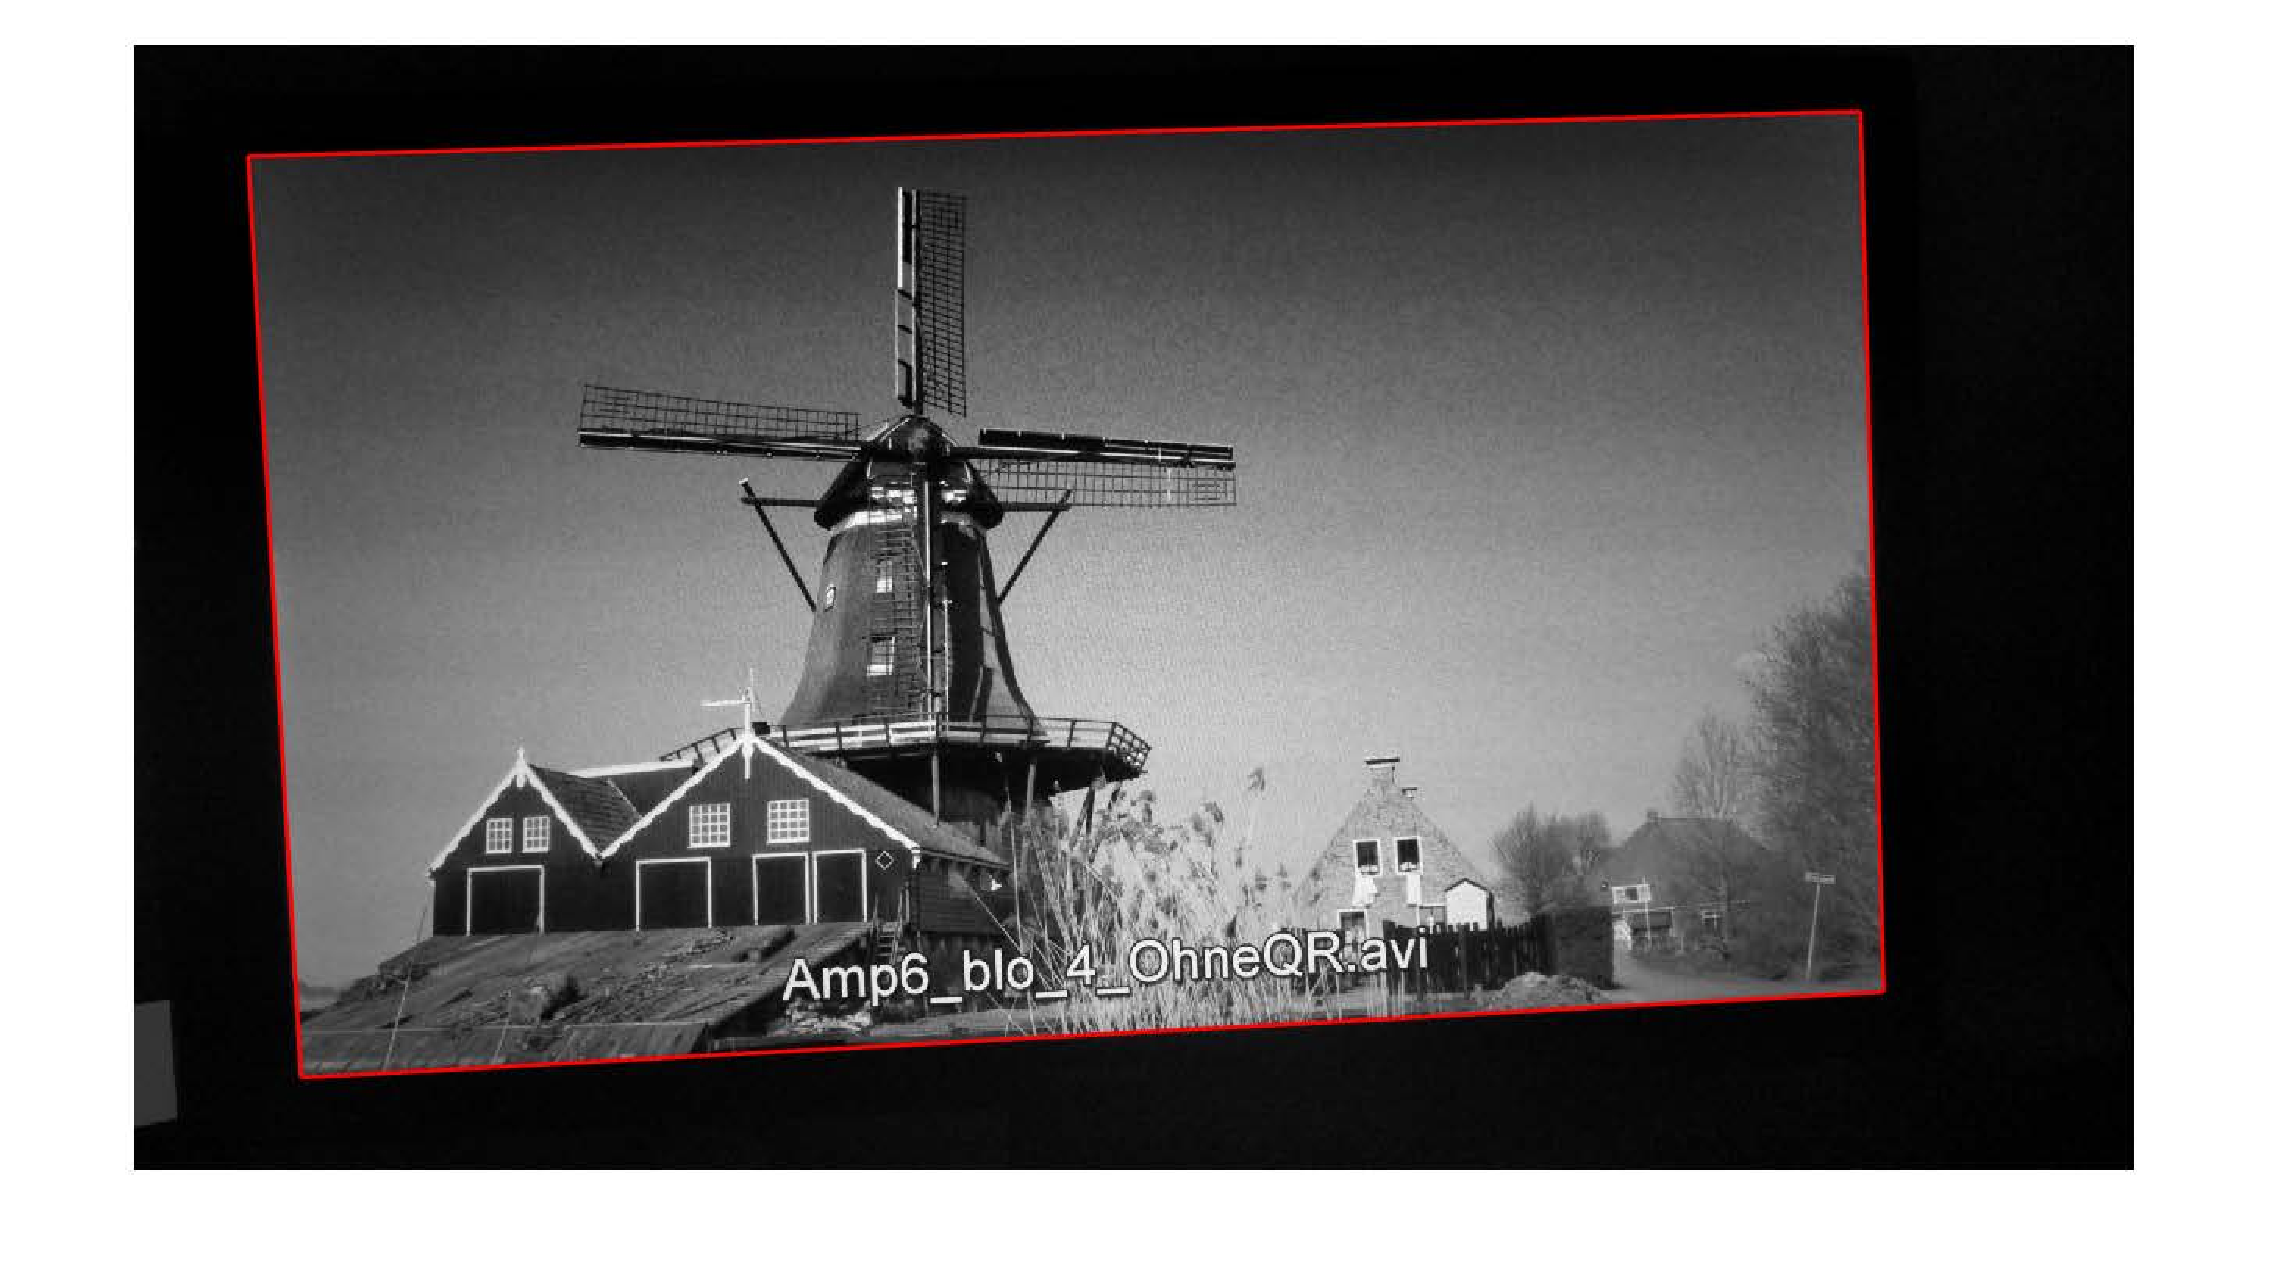
\includegraphics[width=1.0\textwidth]{images/5_Implementirung/2/modulation.pdf}
\caption{Radon Detektion}
\label{fig:radon}
\end{minipage}
\end{figure}

\begin{figure}[H]
 \centering 
  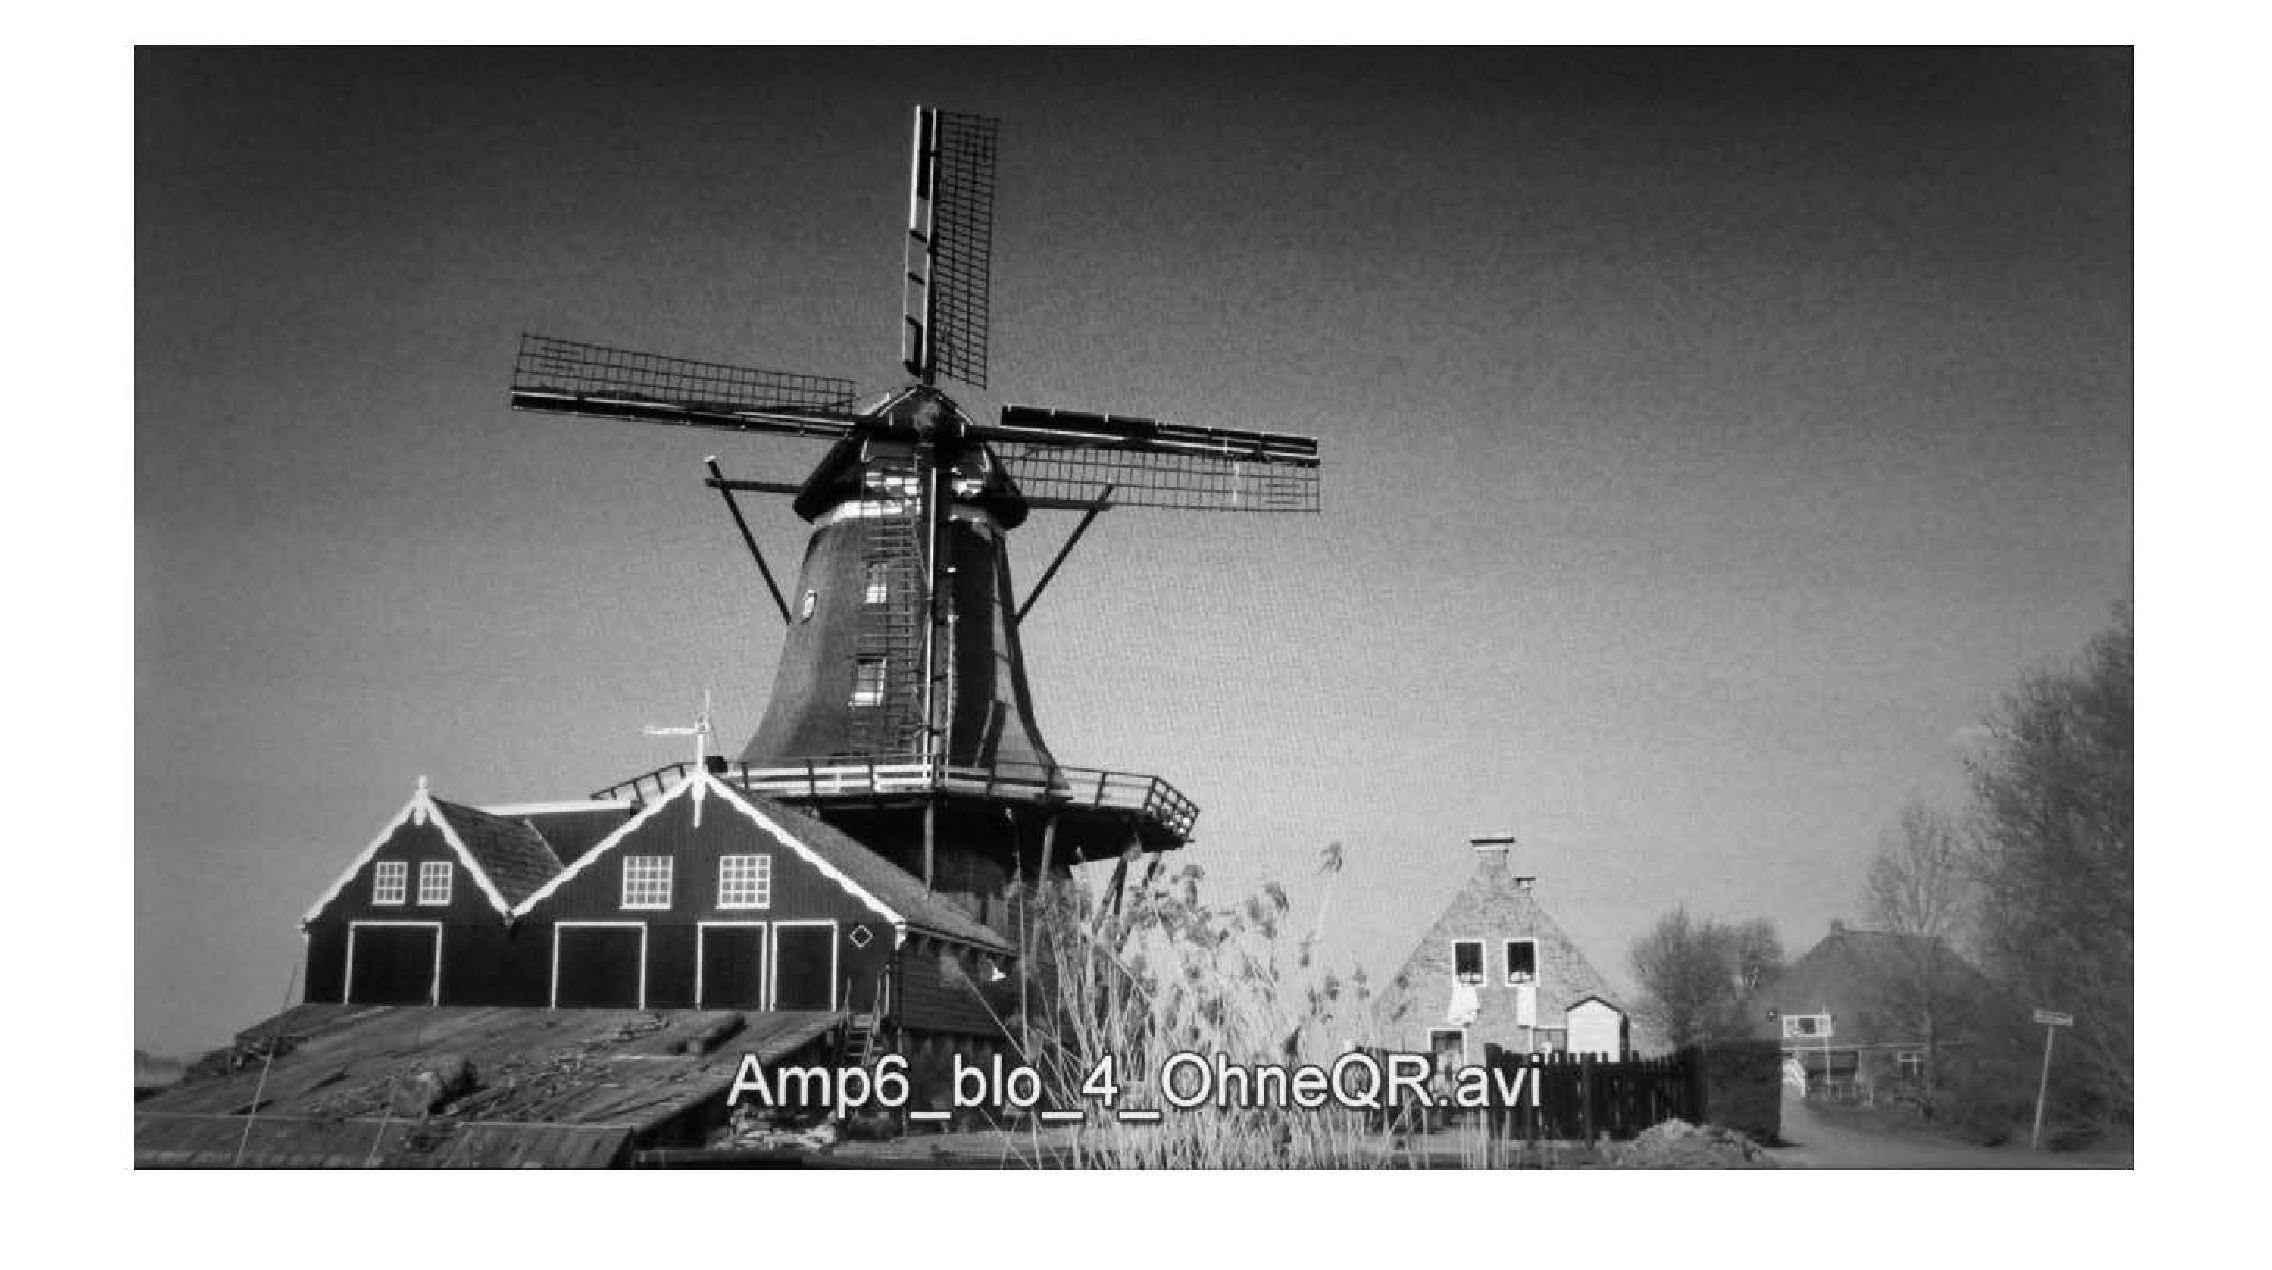
\includegraphics[keepaspectratio,width=1.0\textwidth]{images/5_Implementirung/2/ergebnis.pdf}
 \caption{Ergebnis der 2. Methode}
 \label{fig:Ergebnis1}
\end{figure}

Als Nächst einige Ergebnisse der Verwendungen von die 2. Methode wird angegeben.

Bilder

\section{Implementierung auf einer Smartphone-GPU}

In diese Abschnitt wird die Implementierung auf Smartphone-GPU erläutert. Hier wird Smartphone Xiaomi Mi3 benutzt. Dessen Parameter sind in Tabelle \ref{tbl:Grundlegende Parameter für Mi3} verfügbar. 
Durch RenderScript, als ein Framework für High Performance Computing auf der Android-Plattform, kann die vorherige Methode auf Smartphone-GPU parallel implementiert wird. Die zweite Methode ist hier implementiert. Die verwendet Software auf der PC-Seite läuft Android Studio 3.1.4.

\begin{table}[htb]
	\captionabove{Grundlegende Parameter für Mi3}
	\label{tbl:Grundlegende Parameter für Mi3}
	\footnotesize
	\centering
	\rowcolors{2}{white}{gray!25}	%TUgreen!25
	%\begin{tabular}{|p{2cm}|p{4cm}|p{3cm}|p{3cm}|}	%p{}m{}b{}clr
	\begin{tabular}{|c|c|c|c|}
	\toprule
	\textbf{Smartphone} & \textbf{GPU} & \textbf{CPU} & \textbf{RAM}\\
	\midrule
	Mi3  & Qualcomm Snapdragon 800 MSM8274AB & Krait 400, 2300MHZ & 2 GB, 800 MHZ \\
	\bottomrule
	\end{tabular}
\end{table} 

\textbf{RenderScript}

RenderScript stellt eine native High-Performance-Computing-API bereit, die in C (C99-Standard) geschrieben ist. Mit Renderscript können Anwendungenssoftware automatisch verschiedene Operationen parallel über alle verfügbaren Prozessorkerne ausführen. Es bietet auch Unterstützung für verschiedene Verarbeitungsarten wie CPU, GPU oder DSP. Renderscript ist nützlich für die Grafikverarbeitung, mathematische Modelle oder jede andere Anwendung, die viele mathematische Berechnungen erfordert. Darüber hinaus kann auf alle diese Funktionen zugegriffen werden, um verschiedene Architekturen oder eine unterschiedliche Anzahl von Prozessorkernen zu unterstützen, ohne Code zu schreiben. Es ist auch nicht notwendig, die Anwendungenssoftware für verschiedene Prozessortypen zu kompilieren, da der RenderSkript-Code kompiliert wird, während er auf dem Gerät ausgeführt wird.

Die Vorteile für RenderScript sind wie folgend gelegt:
\begin{enumerate}
 \item Convenience: Renderscript ist für die Ausführung auf vielen Geräten in verschiedenen Prozessor- (CPU-, GPU- und DSP-Instanzen) Architekturen ausgelegt. Alle unterstützten Architekturen sind nicht für jedes bestimmte Gerät spezifisch, da sein Code zur Laufzeit auf dem Gerät kompiliert und zwischengespeichert wird.
 \item Effizient: Renderscript stellt parallel eine Hochleistungs-Computing-API zur Verfügung, die den Kernel über das gesamte Gerät verteilt.
 \item Einfach zu verwenden: Renderscript vereinfacht die Entwicklung, wo dies möglich ist, z. B. das Abbrechen von JNI-Code.
\end{enumerate}

Die Ergebnisse der Implementierung auf MI-3 wird in Abbildung \ref{fig:Ergebnis3} gezeigt.

\begin{figure}[H]
 \centering 
  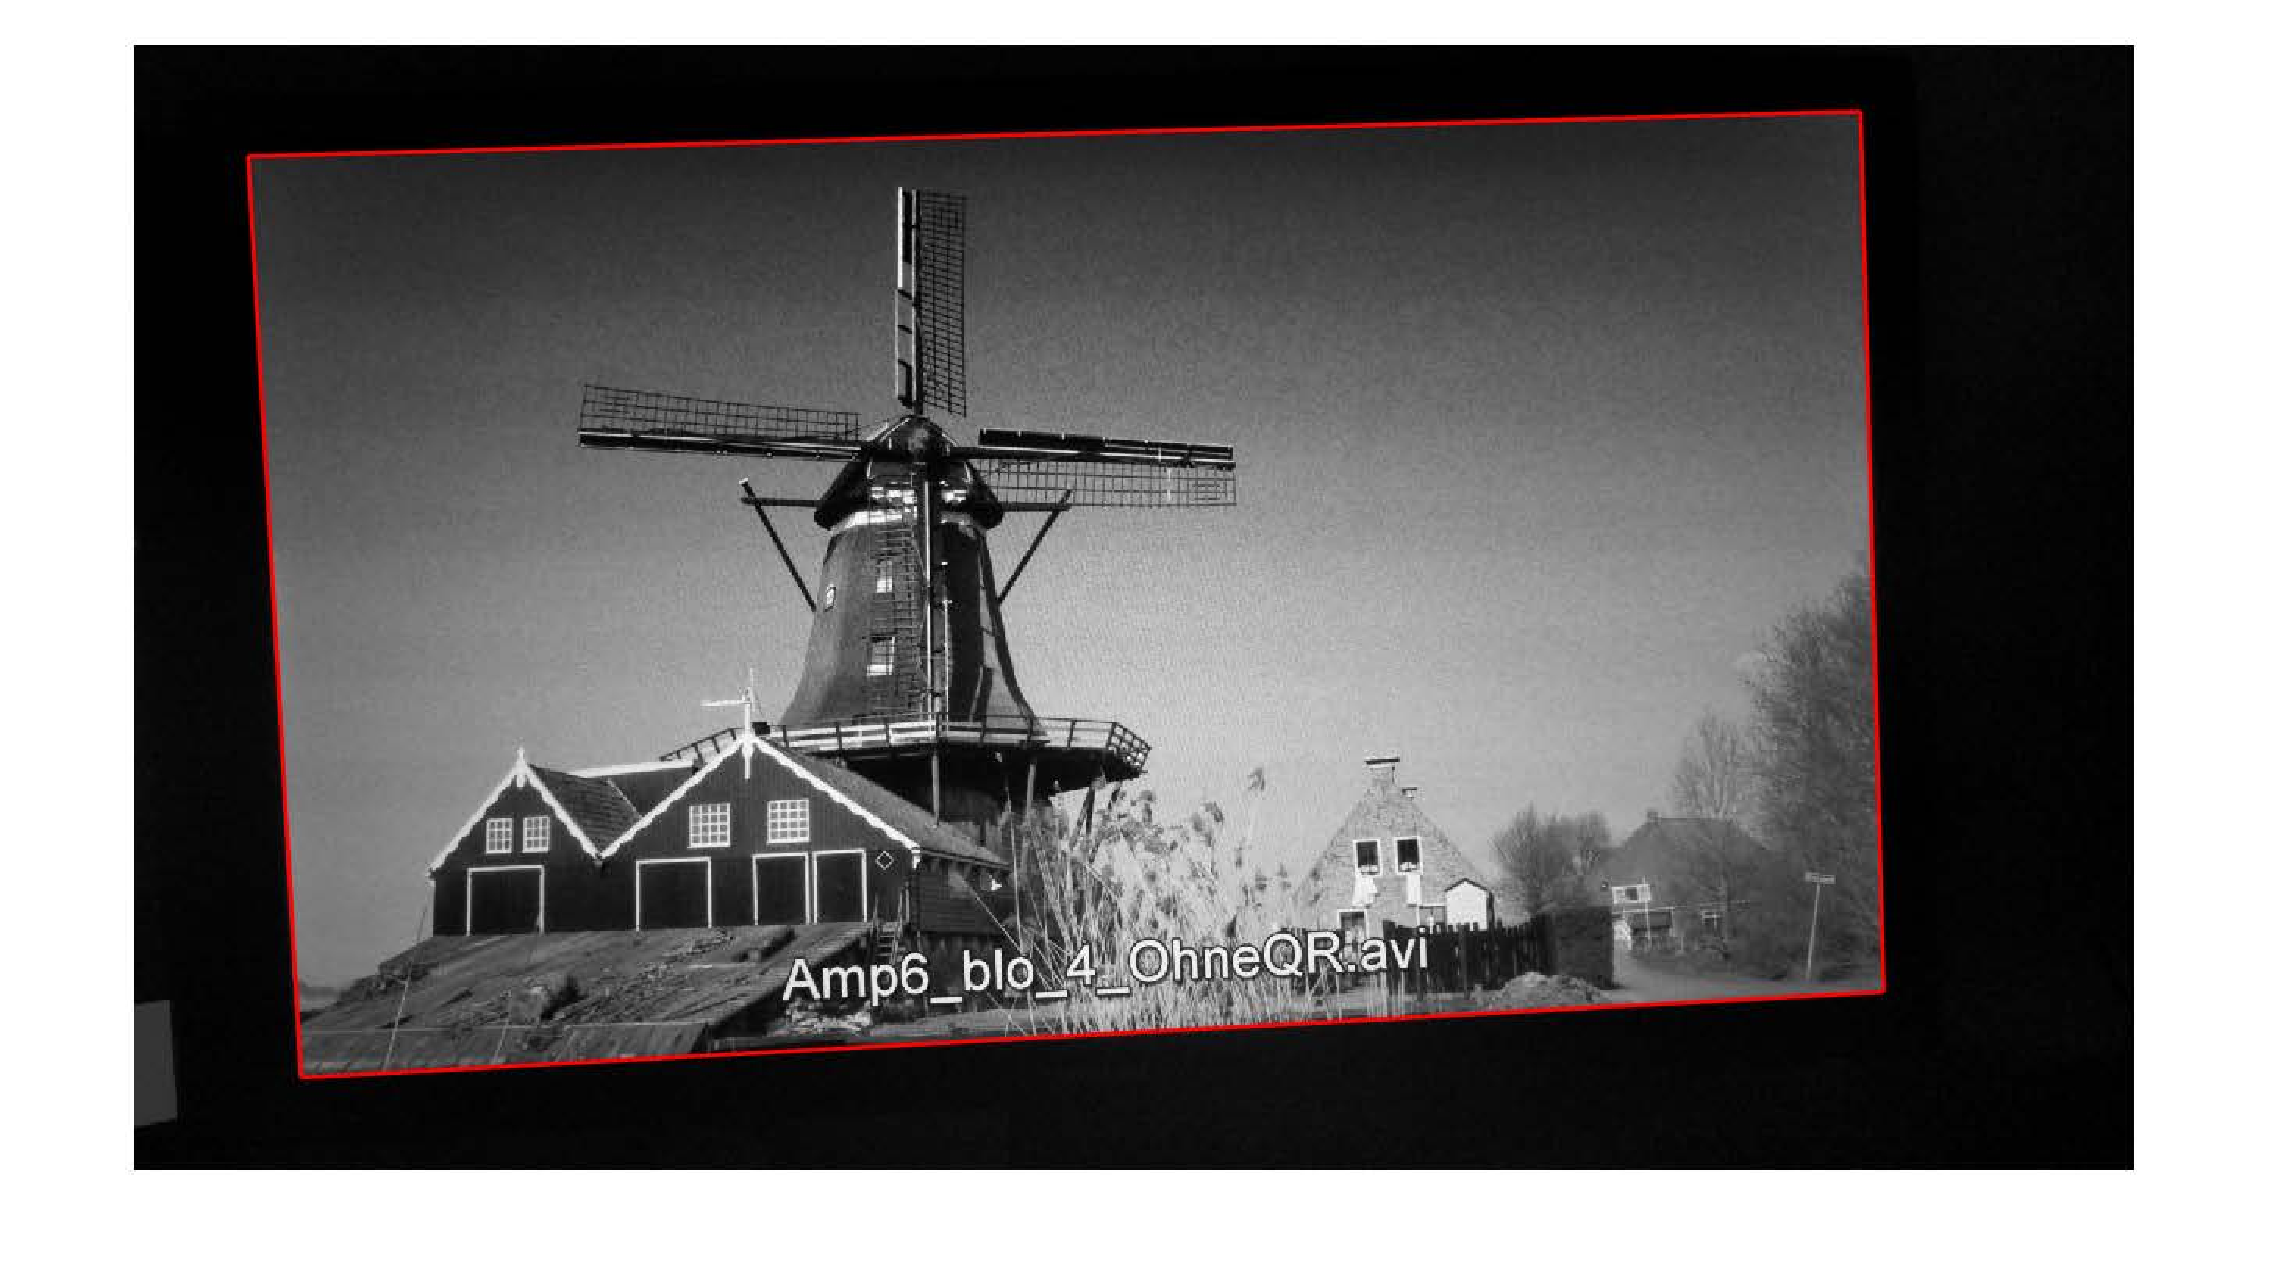
\includegraphics[keepaspectratio,width=1.0\textwidth]{images/5_Implementirung/2/modulation.pdf}
 \caption{Ergebnis auf Smartphone}
 \label{fig:Ergebnis3}
\end{figure}
